\documentclass[bachelor]{thesis-uestc}

\title{基于芯粒库的异构集成芯片设计自动化方法研究}{The Time Marching Scheme of Time Domain
    Integral Equation and Corresponding Fast Algorithm}

\author{郝禹}{Wang Wen}
\advisor{黄乐天\chinesespace 副教授}{Dr. Shengjian Lai}
\school{集成电路科学与工程学院(示范性微电子学院)}{School of Physical Electronics}
\major{微电子科学与工程}{Radio Physics}
\studentnumber{2021020906016}

\begin{document}

\makecover

\begin{chineseabstract}
针对现实复杂环境下芯粒需求定义与验证的难题,本研究提出结构化需求建模与多维度仿真验证方法。通过构建覆盖功能、性能及可靠性指标的映射模型,结合异构集成技术,建立从系统级需求到元器件参数的可回溯验证体系。创新性开发基于OR-Tools的线性规划求解框架,实现功耗、成本等多目标约束下的器件选型优化;设计LegoSim异构仿真平台,集成Gem5、GPGPU-Sim等工具实现松耦合协同仿真,通过迭代收敛机制将时序误差控制在1.8\%以内;构建基于nemu的CPU模拟器,实现简单快速的预仿真。实验结果表明,所提方法支持矩阵乘法、多层感知器等典型任务的混合精度验证。目前该研究已被航天五所应用,具有高度的应用价值。



\chinesekeyword{芯粒,先进封装,微系统,需求建模,异构仿真,线性规划}
\end{chineseabstract}

\begin{englishabstract}
    Faced with the challenges of defining and verifying chiplet requirements in complex real-world environments, this study proposes a structured requirement modeling and multi-dimensional simulation verification method. By constructing a mapping model that covers functional, performance, and reliability metrics, combined with heterogeneous integration technology, a traceable verification system is established from system-level requirements to component parameters. An innovative linear programming solution framework based on OR-Tools is developed to optimize device selection under multi-objective constraints such as power consumption and cost. The LegoSim heterogeneous simulation platform is designed, integrating tools like Gem5 and GPGPU-Sim to achieve loosely coupled co-simulation, with an iterative convergence mechanism controlling timing errors within 1.8\%. A CPU simulator based on nemu is constructed to enable simple and fast pre-simulation. Experimental results show that the proposed method supports mixed-precision verification for typical tasks such as matrix multiplication and multilayer perceptrons. This research has already been applied by the Fifth Academy of Aerospace, demonstrating significant practical value.

\englishkeyword{Chiplet, advanced packaging, microsystem, requirement modeling, heterogeneous simulation, linear programming}
\end{englishabstract}

\thesistableofcontents

\chapter{绪\hspace{6pt}论}

\section{研究工作的背景与意义}

在过去的几十年里,多核处理器克服了“功率墙”难
题\citing{cit1},实现了数量级的效率提高。为了解决“存储墙”问
题\citing{cit2},采用非冯·诺伊曼架构是一个具有前景的解决方
案\citing{cit3,cit4,cit5}。但由于制造良率的下降和先进工艺中每个晶体管
成本的增加,无法以低成本的方式通过大芯片获得高集成
度,“面积墙”已经开始出现。“面积墙”的挑战催生了以多
个小型功能芯片(称为芯粒,chiplet)通过先进封装集成为
一个大规模的系统级集成芯片。

芯粒是指预先制造好、具有特定功能的、可组合集成的裸芯(Die),其功能可包括通用处理器\citing{cit6,cit7,cit8,cit9,cit10,cit11}、存储器、加速
器\citing{cit13,cit14,cit15,cit16}、图形处理器\citing{cit17,cit18,cit19}、I/O接口\citing{cit9}、可编程门阵列\citing{cit20}
等。根据任务需求,将多个具备不同功能的芯粒通过先进
封装技术封装形成一个芯片,这样的芯片称为集成芯片。
由于芯粒都是预先制造好的可用裸芯,相较于传统的单一
芯片不仅面积更小,而且不同功能芯粒还可以使用不同工
艺制造。这些优势综合起来将带来成本的降低。同时复
用这些现成的芯粒可以缩短芯片设计周期。由于基板的
面积要大于光刻区域面积,多芯粒集成技术还可以让集成
芯片不再受限于光刻区域面积的上限,从而构造出面积更
大、功能更加复杂的集成芯片。

芯粒的设计思想仍然采用自上而下的设计方法。首
先,根据应用特征抽象分解成若干标准的芯粒作为功能部
件。这些芯粒都是预先制造好的,之后只需要通过先进封
装组成面向不同应用的集成芯片即可。具体方法如图\ref{pic1}所示。
    \begin{figure}[h]
    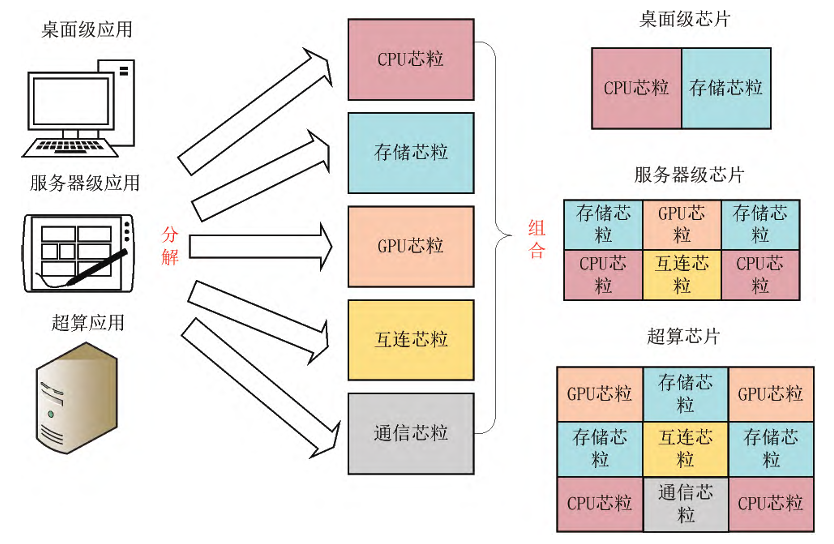
\includegraphics[width=0.5\textwidth]{pic1.png}
    \caption{RWG 基函数几何参数示意图}
    \label{pic1}
    \end{figure}

异构集成芯片设计自动化方法正利用了芯粒设计思想中自上而下的设计方法。目前,对于芯粒的仿真方法一般采用gem5\citing{cit21},gpgpu-sim\citing{cit22},sniper-sim\citing{cit23}这三个仿真模型。

gem5 是一个模块化的计算机体系结构仿真平台,支持多种体系结构(如 x86、ARM、RISC-V 等)和多种仿真模式(如全系统仿真和系统调用仿真)。
特点:
提供灵活的模块化设计,允许用户根据需求定制仿真环境。
支持多核和多线程仿真。
提供详细的硬件行为建模,包括缓存、内存、总线等。
应用场景:
处理器设计与优化。
系统级性能评估。
新型体系结构研究。

GPGPU-Sim 是一个用于通用 GPU (GPGPU) 应用的周期精确仿真器,能够模拟 GPU 的执行行为和性能。
特点:
提供对 CUDA 和 OpenCL 应用的支持。
模拟 GPU 的硬件特性,包括线程调度、内存访问、缓存行为等。
提供详细的性能统计信息。
应用场景:
GPU 架构设计与优化。
GPU 应用性能分析。
新型 GPU 技术研究。

Sniper-Sim 是一个高性能的多核处理器仿真器,专注于并行多核系统的性能建模。
特点:
提供抽象级别较高的仿真模式,能够在保证精度的同时提高仿真速度。
支持多核和多线程仿真。
提供详细的性能分析工具。
应用场景:
多核处理器设计与优化。
并行应用性能分析。
系统级性能评估。

本研究考虑了上述背景,提出了基于芯粒库的异构集成芯片设计自动化方法。该方法通过构建芯粒库,利用线性规划进行器件选型,并结合异构仿真平台实现高效的芯片设计验证。与此同时,该方法还结合了基于nemu的CPU模拟器,实现了简单快速的预仿真。通过这些方法,能够有效地提高芯片设计的效率和准确性。

目前,纵观国内外对于计算机系统的仿真器,往往只聚焦于单一的仿真器,缺乏对多种仿真器的集成与协同仿真。本文提出的异构集成芯片设计自动化方法,正是基于这一背景,旨在实现多种仿真器的集成与协同仿真,从而提高芯片设计的效率和准确性。

该研究已被航天五所应用,具有高度的应用价值。

\section{芯粒设计自动化的研究历史和现状}

芯粒(Chiplet)设计自动化的发展历程可以追溯到20世纪80年代。当时,集成电路设计主要以单一芯片(monolithic IC)为核心,设计自动化工具(EDA)也主要服务于单芯片的电路设计、版图布线和验证。随着摩尔定律逐渐逼近物理极限,芯片面积、功耗和制造良率等问题日益突出,传统的单芯片集成方式面临“面积墙”“功耗墙”等挑战\citing{cit1,cit2}。

为应对这些挑战,业界提出了多芯片集成和异构集成的设计理念。芯粒技术应运而生,通过将多个预先制造、具备不同功能的芯粒(如CPU、GPU、存储器、加速器等)通过先进封装集成到同一系统中,实现高集成度、高灵活性和高可扩展性的系统级芯片(SoC)\citing{cit3,cit4,cit5}。芯粒设计方法采用自上而下的系统级设计思想,先将系统功能分解为标准化芯粒,再通过封装集成满足不同应用需求。这一理念极大地推动了芯片设计的模块化和复用化进程。

在芯粒设计自动化领域,早期的研究主要集中在芯粒接口标准、芯粒间互连、封装技术等底层实现问题。随着技术的进步,研究重心逐步转向芯粒库的构建、芯粒选型优化、系统级协同设计与仿真等高层次自动化方法。例如,近年来出现了基于线性规划的芯粒选型方法\citing{cit12},以及集成多种仿真器(如gem5\citing{cit21}、GPGPU-Sim\citing{cit22}、Sniper-Sim\citing{cit23})的异构仿真平台,用于支持复杂系统的设计空间探索和性能验证。

目前,国内外在芯粒设计自动化方面的研究主要集中在以下几个方向:
\begin{itemize}
    \item \textbf{芯粒库的标准化与复用:} 建立功能完备、接口标准统一的芯粒库,支持不同工艺、不同功能芯粒的灵活组合\citing{cit6,cit7,cit8,cit9,cit10,cit11}。
    \item \textbf{系统级设计与优化:} 采用系统级建模与仿真方法,结合线性规划、启发式算法等手段,实现芯粒选型、互连优化和功耗、性能等多目标约束下的自动化设计\citing{cit12,cit13}。
    \item \textbf{异构仿真与验证:} 集成多种仿真器,实现CPU、GPU、加速器等异构芯粒的协同仿真,提升系统级验证的效率和准确性\citing{cit21,cit22,cit23}。
    \item \textbf{先进封装与互连技术:} 研究2.5D/3D封装、硅中介层、Chiplet互连协议等关键技术,推动芯粒系统的高带宽、低延迟集成\citing{cit9,cit10,cit11}。
\end{itemize}

尽管芯粒设计自动化取得了显著进展,但仍面临芯粒标准化不足、设计工具链不完善、系统级协同优化难度大等挑战。未来,随着芯粒库的不断丰富和设计方法的持续创新,芯粒设计自动化有望在高性能计算、人工智能、云计算等领域发挥更大作用。

\section{本文的主要贡献与创新}
本论文以芯粒库的构建,基于线性规划的芯粒选型方法,基于芯粒库的异构集成芯片设计自动化方法,基于nemu的芯粒模拟方法为重点研究内容,主要创新点与贡献如下:

\begin{enumerate}
\item 依据各个模拟器的特征和芯粒的实际模型构建芯粒库。

\item 基于线性规划的芯粒选型方法,提出了基于OR-Tools的线性规划求解框架,实现功耗、成本等多目标约束下的器件选型优化。

\item 基于legos-sim的异构仿真平台,集成gem5、gpgpu-sim等工具实现松耦合协同仿真,通过迭代收敛机制将时序误差控制在1.8\%以内。

\item 构建并行矩阵运算和MLP两个benchmark,实现不同使用场景下的充分模拟。

\item 基于nemu的CPU模拟器,实现简单快速的预仿真。
\end{enumerate}



\section{本论文的结构安排}
本文共分为五章,各章内容安排如下:

第一章为绪论,介绍了芯粒技术的发展背景、研究意义,综述了国内外在芯粒设计自动化领域的研究现状,明确了本文的主要研究内容和创新点。

第二章为基础研究,系统阐述了芯粒设计自动化的理论基础,包括预仿真模拟器的搭建基础、芯粒库的构建原则、芯粒选型优化方法,以及异构集成芯片设计的系统级建模与仿真流程。

第三章为设计过程,详细介绍了基于芯粒库的异构集成芯片设计自动化方法,重点包括基于nemu的预仿真模拟器使用方法、基于OR-Tools的线性规划芯粒选型方法和仿真自动化流程。

第四章为验证过程和结果,介绍了异构仿真平台的搭建与集成,展示了基于gem5、GPGPU-Sim等仿真器的协同仿真方法,并通过实验验证了所提方法的有效性和优势。

第五章为总结与展望,对全文工作进行了总结,归纳了主要研究成果,并对芯粒设计自动化未来的发展方向和后续工作进行了展望。

\chapter{芯粒设计自动化的基础研究}
本章系统阐述芯粒设计自动化的理论基础与关键技术,为后续的设计实现提供科学依据。首先,从需求定义角度入手,分析了异构集成芯粒的仿真建模方法,探讨了从系统需求到芯粒选择的映射关系,建立了结构化的需求定义模型。其次,深入研究线性规划在芯粒选型中的应用,包括目标函数构建、约束条件设定及基于OR-Tools的求解框架实现,为多目标约束下的芯粒优化提供了数学基础。然后,详细介绍了LegoSim异构仿真平台的架构设计与工作机制,阐述了其松耦合并行架构如何实现高效的多芯粒协同仿真。最后,探讨了NEMU轻量级模拟器的架构与实现,分析了其在预仿真阶段的价值与应用方法。通过这些基础研究,构建了从需求分析、器件选型到性能验证的完整理论体系,为芯粒设计自动化的实际应用奠定了坚实基础。

\section{芯粒库的构建-芯粒需求定义模型}
对于要设计一个异构集成芯粒,如何从系统指标需求出发,在一个具有多种不同功能的芯粒库集合中挑选出合适的型号进行选择,是首先需要解决的问题。需求定义模型的建立可以得到有关芯粒库多方面的指标,为芯粒的选择提供了数据参考。

\subsection{异构集成芯粒的仿真建模综述}
随着处理器设计、验证、制造和管理成本的不断攀升,为特定应用程序设计可行的系统数量受到巨大压力。设计和制造大量片上系统(SoC)的方式变得越来越不可行。得益于新兴的设计和组装方法(如Embedded Multi-Die Interconnect Bridge,EMIB)的开发和商业化,一个大型的处理器SoC现在可以被分解为多个更小的芯粒(Chiplet)组件。这些不同的芯粒可以通过类似SoC的低延迟和高带宽互连的基板连接,重新集成为一个完整的处理器系统。
\subsubsection{Chiplet技术的优势与挑战}

\textbf{优势:}
\begin{itemize}
    \item \textbf{更高的良率:} 较小尺寸的芯粒相比大型SoC更容易制造,降低了缺陷率,提高了生产良率。
    \item \textbf{降低系统成本:} 多个芯粒可以共享设计和制造成本;不同的芯粒可基于不同的工艺节点制造,优化成本结构。
    \item \textbf{实现异构设计:} 能够集成不同功能和特性的芯粒,实现异构系统设计,满足多样化需求。
    \item \textbf{低成本的硬件定制:} 针对不同的应用程序,可以选择不同的芯粒组合,快速构建定制化系统。
\end{itemize}

\textbf{挑战:}
\begin{itemize}
    \item 然而,随着芯粒数量的增多,如何确定设计和制造所需的最小芯粒集,以提供接近定制化的系统性能,成为一个亟待解决的问题。这需要从系统指标需求出发,在多种不同功能的芯粒库中挑选出最合适的组合。
\end{itemize}

\subsubsection{Chiplet成本模型}
一次性开销(Nonrecurring Engineering Cost, NRE) 与 非一次性开销(Recurring Engineering Cost, RE) 是衡量芯粒成本的两个重要维度。
NRE成本:包括体系结构设计、RTL设计、IP验证、物理设计、原型制作、验证和掩模制造等。


RE成本:主要涉及晶圆制造成本,受产率和工艺复杂性影响。


A quantitative cost model and multi-chiplet architecture exploration\citing{cit27}一文中提出了 Chiplet Actuary 成本模型,基于三种典型的多芯片集成技术:多芯片模块(Multi-Chip Module, MCM)、系统级封装(System-in-Package, SiP)、集成扇出型封装(Integrated Fan-Out, InFO)该模型将芯片分为模块、芯粒和封装三个部分,各部分根据不同公式计算总的NRE和RE成本,如\ref{pic2}所示:
\begin{figure}[h]
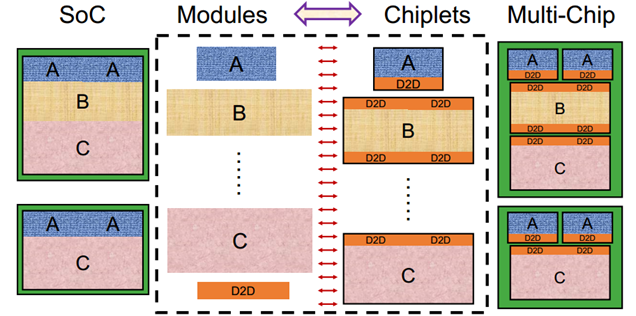
\includegraphics[width=0.5\textwidth]{pic2.png}
\caption{Chiplet模型}
\label{pic2}
\end{figure}

A Toolchain for Rapid Design Space Exploration of Chiplet Architectures\citing{cit26}提出的 RapidChiplet 工具链,主要计算了单个芯粒的制造成本(RE成本)。通过晶圆面积、缺陷密度和良率等数据,精确估算单个芯粒的制造成本。
需要注意的是,最小化芯粒数量并不一定导致总成本最小化。上文提出了基于芯粒组装的成本模型,引入芯粒数量参数来平衡RE和NRE成本之间的关系,从而优化成本。


\subsubsection{Chiplet热模型}
热特性是芯粒系统设计中的重要考虑因素。
An efficient thermal model of chiplet heterogeneous integration system for steady-state temperature prediction\citing{cit25}一文中提出了一种有效的热模型,用于预测芯粒异构集成(Chiplet Heterogeneous Integration,CHI)2.5D系统的稳态温度分布。该模型被评估为高度准确(误差 <1.8\%)且计算速度快,可用于大规模热仿真,帮助设计人员在早期检测温度热点,提高系统的可靠性和鲁棒性。
\begin{figure}[h]
    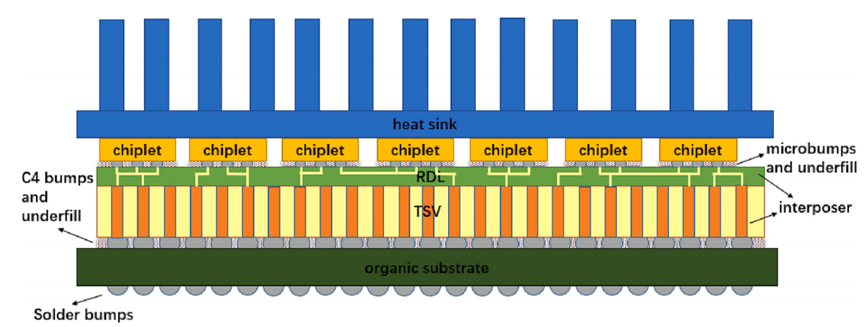
\includegraphics[width=0.7\textwidth]{pic3.png}
    \caption{2.5D系统模型}
    \label{pic3}
    \end{figure}


\subsubsection{Chiplet内部通信仿真}
高效的内部通信对于芯粒系统的性能至关重要。
RapidChiplet 工具链:可以预测芯粒内部互连(Inter-Chiplet Interconnect,ICI)的延迟和吞吐量。其架构如下:
\begin{figure}[h]
    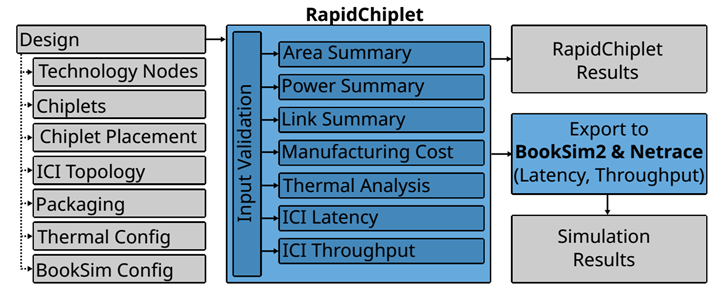
\includegraphics[width=0.7\textwidth]{pic4.png}
    \caption{2.5D系统模型}
    \label{pic4}
    \end{figure}


    工具链将内部通信分为四种类型:计算单元到计算单元(Compute-to-Compute,C2C)、计算单元到存储器(Compute-to-Memory,C2M)、计算单元到I/O(Compute-to-IO,C2I)、存储器到I/O(Memory-to-IO,M2I)。通过最短路径算法计算各路径的延迟和吞吐量,为系统设计提供参考。
    其中提出了事务级建模,通过抽象通信细节,关注数据传输的功能,实现了系统组件之间的高效建模。虽然主要针对片上系统(SoC),但对于芯粒内部总线通信的建模具有借鉴意义。
    

\subsubsection{Chiplet执行程序仿真}
对于需要运行软件的芯粒,执行程序的仿真至关重要。


The next generation of virtual prototyping: Ultra-fast yet accurate simulation of hw/sw systems\citing{cit24}一文中提出了针对需要执行的目标程序的仿真。在这种技术中,目标程序的源代码直接被编译成可以在主机计算机上运行的二进制程序。另外,类似于二进制转换技术,源代码可以根据目标体系结构被赋予一个基于时间和功耗的模型。由于这些仿真是高效的,它们直接在主机计算机上执行目标程序,非常适合系统级设计空间探索。


然而,在这个抽象级别上,准确捕捉复杂的微体系结构行为,如流水线和缓存行为,是困难的。这种仿真方法的另一个缺点是需要访问目标程序的源代码。


\subsubsection{小结}
本节综述了与芯粒仿真建模相关的关键技术,包括成本模型、热模型、内部通信仿真和执行程序仿真。这些仿真工具和方法为芯粒库的选择提供了重要的数据参考,确保在系统设计初期就能够评估不同芯粒组合的性能、成本和可靠性。


进一步来说,对于芯粒的面积、功耗、链路长度等物理参数,通常通过直接测量或简单计算即可获得。本文重点关注通过仿真建模获取难以直接测量的指标,为需求定义模型的理论论证奠定基础。 

\subsection{需求定义现有发展趋势}
近年来,集成电路领域取得了显著进展,推动了尺寸缩小与性能提升、能效优化、多核与异构计算以及物联网与智能化的发展方向和趋势。


在尺寸缩小与性能提升方面,集成电路的制程工艺不断突破,例如3nm制程工艺的推出,使得集成电路的密度和速度得到了显著提升。高密度、高性能的芯粒技术对需求定义提出了更高的要求,需要考虑更高的性能指标和更严格的质量控制标准。


能效优化也是芯粒技术的重要研究方向之一。通过优化电路设计和材料选择,芯粒技术在降低能耗方面取得了显著进展,这要求需求定义中包含能效优化的具体目标和措施。采用低功耗设计策略、先进的功率管理技术,使得芯粒能够在减少能耗的同时保持高效运行。


多核与异构计算的发展使得芯粒能够处理更复杂的计算任务。这种技术路线不仅提高了计算效率,还增强了系统的灵活性和可扩展性。因此在需求定义中,需要考虑多核系统的计算效率、任务分配和资源管理等因素,并考虑异构集成方式因素,以让其满足复杂计算任务的需求。


物联网与智能化的快速发展使得芯粒技术在传感器、通信和数据处理等方面得到了广泛应用。我们需要分析型号电子系统功能、性能以及可靠性需求,以让其能满足用户所提出的要求。


总之,集成电路领域技术的发展对于芯粒的需求定义产生了深远的影响。因此在需求定义中,必须综合考虑尺寸缩小与性能提升、能效优化、多核与异构计算等多个方面的发展需求,以确保芯粒的高效性能和创新应用。


\subsection{现有需求定义模型}
目前,不同领域的需求定义模型在各自项目成功中扮演着关键角色,因此为有效管理项目,提升产品质量,选择适宜的需求定义模型至关重要。目前,广泛应用的需求定义模型包括瀑布模型、敏捷模型、螺旋模型和迭代增量模型等。


瀑布模型(Waterfall Model)作为最早提出的软件开发模型之一,强调过程的线性和顺序性。整个开发流程被划分为需求分析、设计、实现、测试和维护等阶段,每一阶段都有明确的目标和文档输出。其优势在于结构清晰、易于管理和控制,特别适用于需求明确且稳定的项目。然而,瀑布模型的缺陷在于缺乏灵活性,一旦进入下一阶段,返回修改前一阶段的成本高昂,对需求变化的响应能力较弱。在芯粒开发中,如果项目需求稳定且预期变动较小,瀑布模型依然是一个有效的选择。然而,随着芯粒技术的迅速发展,需求的不确定性增加,单纯依赖瀑布模型可能无法满足复杂项目的需求。

\begin{figure}[h]
    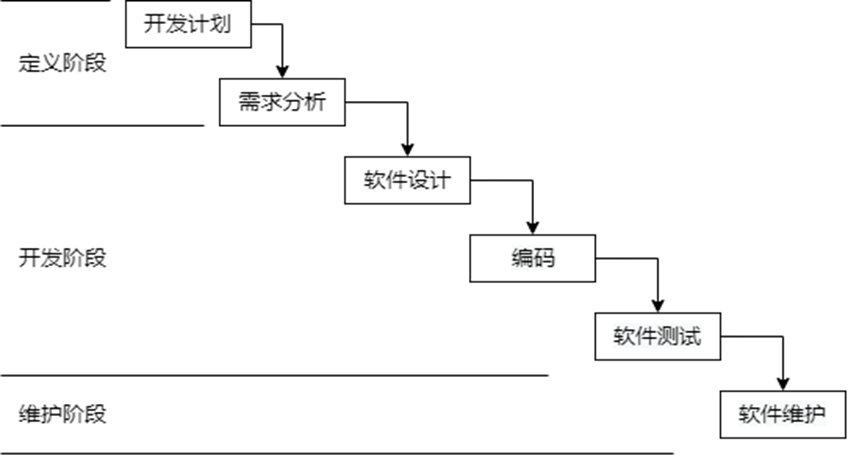
\includegraphics[width=0.5\textwidth]{pic5.png}
    \caption{瀑布模型}
    \label{pic5}
    \end{figure}


敏捷模型(Agile Model)则注重快速迭代和持续交付,通过短周期的迭代不断完善产品。团队与客户保持紧密合作,能够及时响应需求变化,强调团队协作和个人互动。敏捷模型的优势在于高度灵活性和对需求变化的快速响应,适用于需求不明确或经常变化的芯粒项目。例如,在开发新型微机电系统(MEMS)传感器时,市场需求可能迅速变化,采用敏捷模型能够更好地适应这种动态环境。然而,敏捷模型对团队要求较高,需要成员具备自我管理和高效协作的能力。在大型复杂的芯粒项目中,可能会面临协调困难和项目控制挑战。


\begin{figure}[h]
    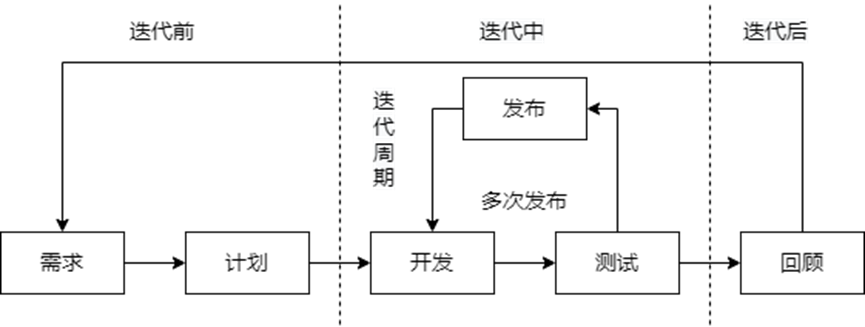
\includegraphics[width=0.5\textwidth]{pic6.png}
    \caption{敏捷模型}
    \label{pic6}
    \end{figure}

V模型(V-Model)是一种强调验证和确认的开发模型,与瀑布模型类似,但在每个开发阶段都对应了相应的测试阶段。此模型确保在开发的每个阶段都进行充分的验证,从而提高产品的质量和可靠性。对于医疗器械、航空航天等对质量和安全性要求极高的芯粒项目,V模型能够提供严格的质量保障。然而,其缺点在于缺乏灵活性,变更成本高,开发周期较长,可能不适用于需求频繁变化的项目。

\begin{figure}[h]
    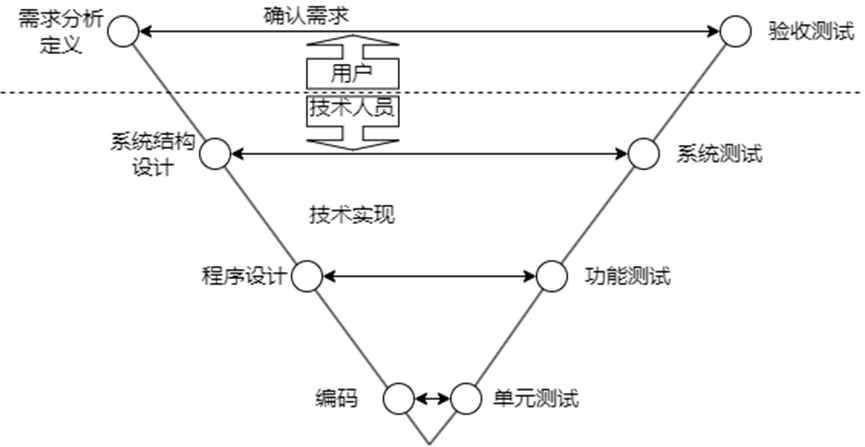
\includegraphics[width=0.5\textwidth]{pic7.png}
    \caption{V模型}
    \label{pic7}
    \end{figure}

螺旋模型(Spiral Model)结合了瀑布模型和迭代模型的特点,特别强调风险分析和管理。每次迭代都经过计划、方案设计、工程评估和开发验证四个阶段,逐步完善系统。螺旋模型适用于大型、复杂且具有高风险的芯粒项目,能够有效管理项目的不确定性和技术风险。例如,在开发高精度芯粒集成电路时,技术风险和市场风险较高,螺旋模型可以帮助团队提前识别和应对这些挑战。然而,该模型成本较高,对团队的风险分析能力要求较高,需要有经验的专业团队支持。

\begin{figure}[h]
    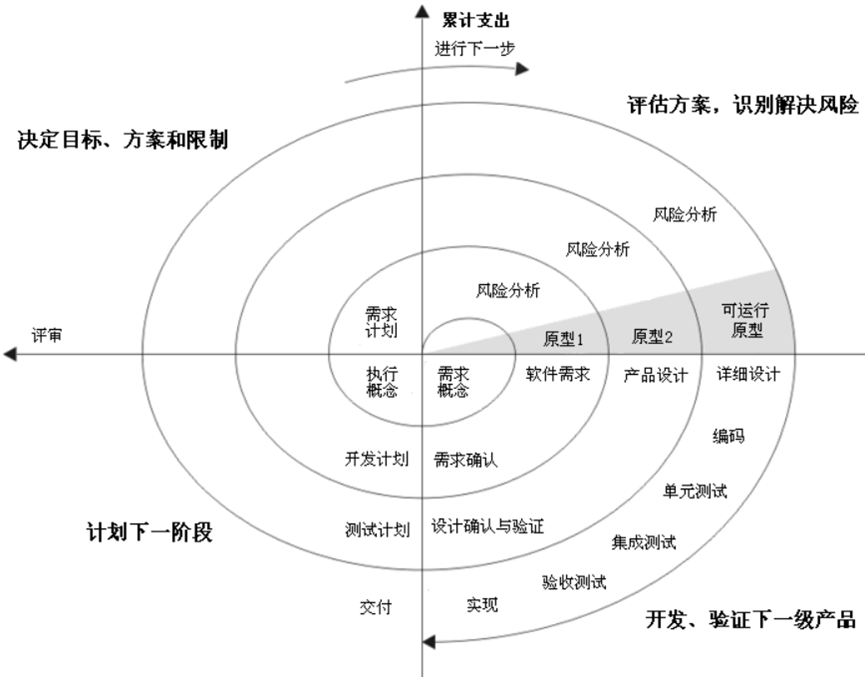
\includegraphics[width=0.5\textwidth]{pic8.png}
    \caption{螺旋模型}
    \label{pic8}
    \end{figure}

迭代增量模型(Iterative and Incremental Model)将开发过程划分为若干小的增量,每个增量都是一个可交付的部分产品,以此逐步构建完整系统。其优势在于能够逐步交付产品功能,持续获得客户反馈,降低项目风险。对于需求逐步明确的芯粒项目,如新技术的探索性开发,迭代增量模型能够提供灵活的开发方式。然而,该模型需要良好的整体规划和架构设计,确保各增量之间的无缝集成,否则可能导致系统架构不统一、维护成本增加的问题。

\begin{figure}[h]
    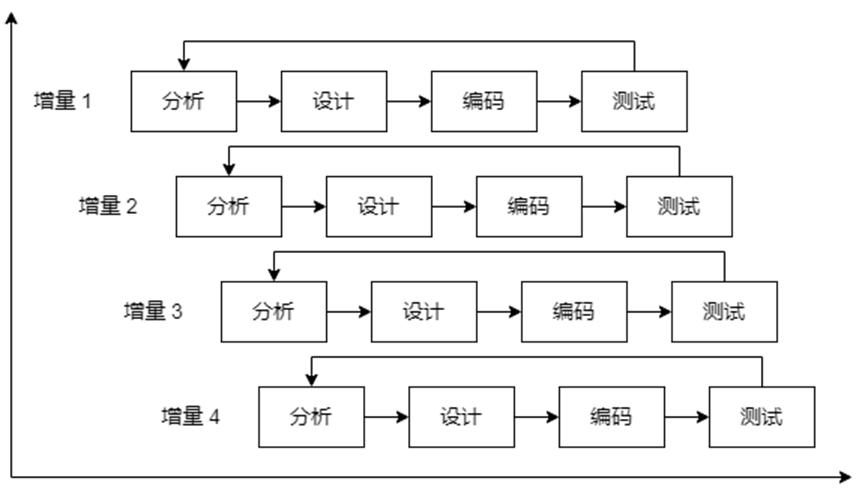
\includegraphics[width=0.5\textwidth]{pic9.png}
    \caption{迭代增量模型}
    \label{pic9}
    \end{figure}

在芯粒工程项目中,需求定义模型的选择应综合考虑项目规模、复杂性、需求的确定性、团队能力以及项目风险等多种因素。例如,随着集成电路工艺向3nm及以下节点演进,工艺复杂度和技术风险显著增加,采用螺旋模型可能更有利于风险管理和技术突破。对于物联网领域的芯粒开发,需求变化快、市场响应速度要求高,敏捷模型能够提供更大的灵活性和快速交付能力。
此外,现代芯粒的发展趋势如系统级封装(SiP)、片上系统(SoC)以及异构集成等,也对需求定义模型提出了新的要求。面对多学科融合、高度集成的芯粒产品,传统的开发模型可能无法有效应对,需要结合多种模型的优势,甚至探索新的需求定义方法。例如,在SoC设计中,需要同时考虑硬件、软件以及固件的协同开发,可能需要结合敏捷模型的迭代性和V模型的验证机制,确保产品的质量和性能。

\begin{table}[h]
\caption{需求定义模型比较}
\centering
\begin{tabular}{p{2.5cm}p{3.5cm}p{4cm}p{3.5cm}}
\toprule
\textbf{模型} & \textbf{优点} & \textbf{缺点} & \textbf{适用场景} \\
\midrule
瀑布模型 & 结构清晰,阶段分明 & 缺乏灵活性,响应变更能力弱,风险后置 & 需求明确且稳定的项目 \\
敏捷模型 & 高度灵活性,客户参与度高 & 对于团队要求高,大型项目协调难度大 & 创新性强、需要快速试错的开发 \\
V模型 & 质量保证好,验证过程清晰 & 缺乏灵活性,开发周期长 & 质量和安全性要求高的项目 \\
螺旋模型 & 风险驱动,迭代开发 & 成本高,项目周期较长 & 大型、复杂且高风险的项目 \\
迭代增量模型 & 逐步交付,灵活性高,风险分散 & 整体规划复杂,集成难度高 & 需求逐步明确的项目 \\
\bottomrule
\end{tabular}
\label{tab:requirement_models}
\end{table}

\subsection{芯粒需求定义模型的合理性分析}
芯粒技术的迅猛发展,对需求定义模型提出了更高的要求。合理的需求定义模型能够有效指导芯粒项目的成功实施,提升系统性能和可靠性。结合现有模型和技术路线,分析芯粒需求定义模型的合理性,对于推动芯粒领域的创新具有重要意义。


芯粒的技术路线涵盖了尺寸缩小与性能提升、能效优化、多核与异构计算、物联网与智能化等前沿领域。这些技术路线的特性要求需求定义模型具备灵活性、可靠性和适应性,以应对技术不确定性和市场需求的不断变化。传统的需求定义模型,如瀑布模型、敏捷模型、V模型、螺旋模型和迭代增量模型,各自具有独特的优势。当我们将这些模型与芯粒的技术路线相结合,可以更好地满足项目需求,确保项目的成功推进。


然而,单一的需求定义模型可能无法全面满足芯粒项目的复杂需求。因此,将不同模型的优势相结合,形成一种复合的需求定义模型,是一种更为合理的选择。比如,在项目的早期阶段采用敏捷模型,快速迭代,获取用户反馈,及时调整开发方向;在涉及关键功能和安全性的部分,引入V模型的验证机制,确保系统的可靠性和稳定性。


而对于项目所提出的分析型号电子系统功能、性能及可靠性需求,建立从型号电子系统到宇航SoC、ASIC、SiP、连接器的功能、性能及可靠的映射关系,形成结构化的需求映射,建立需求模型。再建立电子系统一元器件指标的回溯模型,验证系统需求与元器件需求的对应关系,检验需求定义模型的正确性。可以结合上述需求定义模型进行分析。


利用瀑布模型其强调线性、顺序的开发流程,从需求分析、设计、实现到测试和维护,每个阶段都有明确的任务。在芯粒需求定义模型的构建中,瀑布模型提供了一个清晰的框架。团队可以按照固定的步骤,先全面分析型号电子系统的功能、性能及可靠性需求,然后依次建立从系统到宇航级SoC、ASIC、SiP、连接器等元器件的功能、性能及可靠性的映射关系,形成结构化的需求模型。但其要求中的回溯模型由于其线性性质难以适配。


若是后续再利用V模型其强调验证和确认过程的特性,其与芯粒需求定义的回溯模型密切相关。在建立需求模型后,V模型要求在每个开发阶段都进行相应的测试和验证。通过建立电子系统到元器件指标的回溯模型,团队可以验证系统需求与元器件需求的对应关系,确保需求定义模型的正确性。每个元器件的指标和功能都需要经过验证,确保符合系统的功能、性能和可靠性需求,从而正确的实现项目开展。结合以上两个模型,便能够更好的实现预期的需求要求。


\begin{figure}[h]
    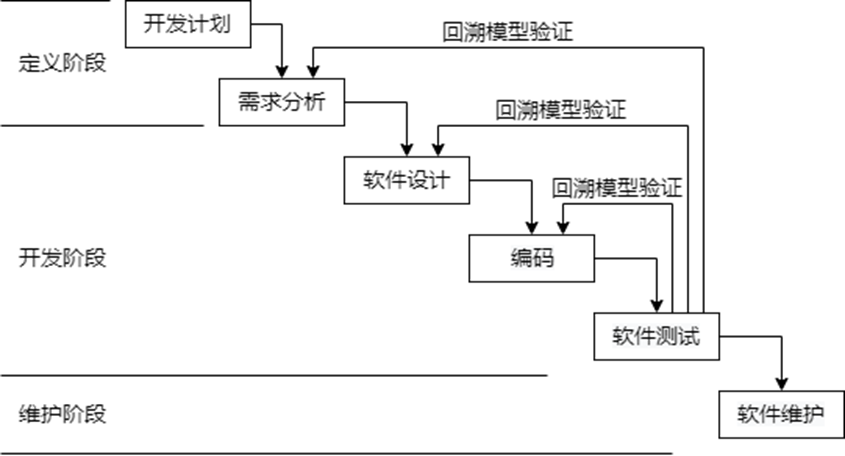
\includegraphics[width=0.5\textwidth]{pic10.png}
    \caption{需求定义模型}
    \label{pic10}
    \end{figure}


\subsection{小结}
本节综合性地通过灵活运用和组合不同的需求定义模型,既能确保需求定义的全面性和准确性,又能提高对变化的响应能力和对风险的控制能力。说明构建合理的芯粒需求定义模型,不仅是理论上的必要,也是实践中取得成功的关键。

\section{仿真器的线性规划}

线性规划作为一种关键的数学优化技术,在众多领域发挥着举足轻重的作用,其应用范围之广、影响力之大,使其成为解决复杂问题的有力工具。线性规划问题是在一组线性约束条件下,寻求一个线性目标函数的最大值或最小值。这种问题的提出源于现实世界中对资源的合理配置、生产计划的优化、成本的最小化等诸多需求。一个线性规划问题主要有目标函数,约束条件等基本要素构成。

\subsection{目标函数}
目标函数是线性规划问题的关键,其清晰地指明了优化的方向。在数学形式上,目标函数是一个关于决策变量的线性表达式,通常表示为 $Z=c_1 x_1+c_2 x_2+\cdots+c_n x_n$,其中 $Z$ 代表目标函数值,$c_1$, $c_2$,$\ldots$,$c_n$ 是决策变量 $x_1$, $x_2$,$\ldots$,$x_n$的系数,这些系数反映了各个决策变量在目标函数中的重要程度或贡献大小。例如,在一个投资组合问题中,目标函数可能是最大化投资收益,决策变量 $x_1$, $x_2$,$\ldots$,$x_n$ 分别代表在不同投资项目上的投资金额,系数 $c_1$, $c_2$,$\ldots$,$c_n$ 则对应各投资项目的预期收益率。通过对目标函数的优化,可以在满足约束条件的前提下,找到使目标函数值达到最大(或最小)的决策变量取值组合,从而实现资源的最佳配置和目标的最优达成。约束条件是限制决策变量取值范围的线性不等式或等式。这些约束条件通常来源于实际问题中的资源限制、生产能力限制、市场需求限制等因素。


\subsection{约束条件}
约束条件是线性规划问题的框架,它界定了决策变量的可行取值范围,确保问题的解决方案在实际应用中具有可行性和合理性。约束条件通常由一组线性不等式或等式构成,形式为 $a_{11} x_1+a_{12} x_2+\cdots+a_{1n} x_n \leq(\geq, =) b_1$,$a_{21} x_1+a_{22} x_2+\cdots+a_{2n} x_n \leq(\geq, =) b_2$,$\ldots$,$a_{m1} x_1+a_{m2} x_2+\cdots+a_{mn} x_n \leq(\geq, =) b_m$,其中 $a_{ij}$ 是约束条件的系数,$b_i$ 是约束条件的常数项,$m$ 表示约束条件的个数。

\subsection{线性规划问题的求解方法}
\subsubsection{图解法}
图解法适用于只有两个决策变量的线性规划问题。通过在二维坐标系中绘制约束条件所表示的区域,找到可行解区域,再根据目标函数的等值线确定最优解。该过程如图\ref{pic11}所示。
\begin{figure}[h]
    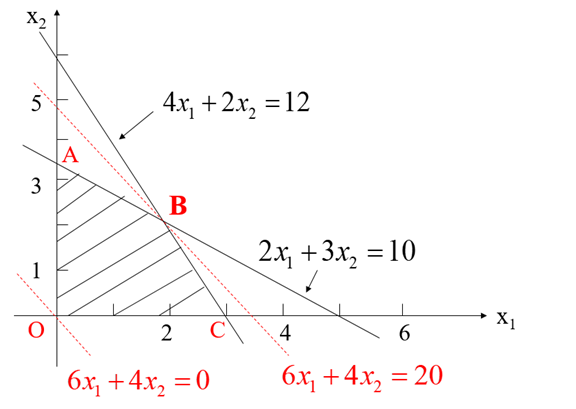
\includegraphics[width=0.5\textwidth]{pic11.png}
    \caption{图解法示意图}
    \label{pic11}
    \end{figure}

    \subsubsection{单纯形法}
    单纯形法是解决线性规划问题最常用的方法之一,适用于多个决策变量的情况。它从可行解区域的一个顶点出发,沿着目标函数值递增(或递减)的方向,逐步移动到相邻的顶点,直到找到最优解。
    
    单纯形法的基本步骤如下:
    \begin{enumerate}
        \item 将线性规划问题转化为标准形式,即目标函数为最大化,约束条件为等式,且所有变量非负。
        \item 构造初始单纯形表,确定初始基可行解。
        \item 检查目标函数的系数,判断是否达到最优解。如果所有非基变量的检验数(目标函数系数减去对应的约束系数乘以基变量的检验数之和)都小于等于 0(对于最大化问题),则当前基可行解为最优解;否则,选择检验数最大的非基变量作为进基变量。
        \item 确定离基变量,即在保持基可行解的前提下,使进基变量的值增加最多的那个基变量。
        \item 进行基变换,更新单纯形表,重复步骤 3 和 4,直到找到最优解。
    \end{enumerate}
    该过程的流程图如图\ref{pic12}所示。
    
    \begin{figure}[h]
        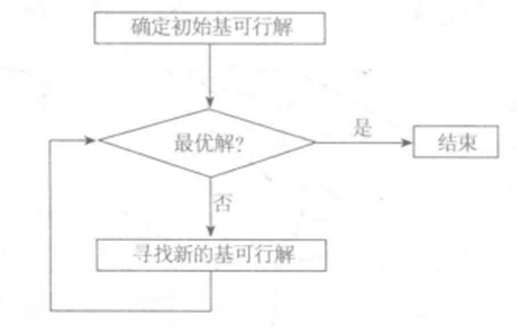
\includegraphics[width=0.5\textwidth]{pic12.png}
        \caption{单纯形法流程图}
        \label{pic12}
    \end{figure}

\subsubsection{对偶单纯形法}
对偶单纯形法是单纯形法的一种变体,它从对偶问题的角度出发求解线性规划问题。对偶问题与原问题有着密切的联系,通过对偶问题的求解可以得到原问题的最优解。


对偶单纯形法的基本思想是:从原问题的一个不可行但目标函数值较好的解出发,通过调整约束条件的右端项,使其逐渐变得可行,同时保持目标函数值不劣于当前值,直到找到原问题的最优解。

\subsection{整数线性规划问题及其求解方法}
整数线性规划是线性规划的一种扩展形式,它要求决策变量取整数值。整数线性规划的求解方法比线性规划复杂,因为整数约束使得问题的可行解集不再是一个简单的多面体,而是一个离散的点集。
\subsubsection{分支定界法}
分支定界法是一种常用的求解整数线性规划问题的方法。其基本步骤如下:
\begin{enumerate}
    \item 首先求解整数线性规划问题的松弛问题,即去掉整数约束后的线性规划问题,得到一个下界(对于最大化问题)或上界(对于最小化问题)。
    \item 选择一个非整数解的决策变量,将其取值范围分成两个子区间,分别对应该变量取整数值的两个相邻整数,从而将原问题分解为两个子问题。
    \item 对每个子问题重复步骤 1 和 2,不断分支,同时记录每个子问题的目标函数值和可行解。
\end{enumerate}

在分支过程中,如果某个子问题的目标函数值超过了已知的最优目标函数值(对于最大化问题)或小于已知的最优目标函数值(对于最小化问题),则可以剪掉该子问题的分支,因为该分支不可能产生更好的解。

当所有分支都被探索完毕或达到一定的迭代次数时,记录的目标函数值最大的(或最小的)可行解即为整数线性规划问题的最优解。该过程如图\ref{pic13}所示。

\begin{figure}[h]
    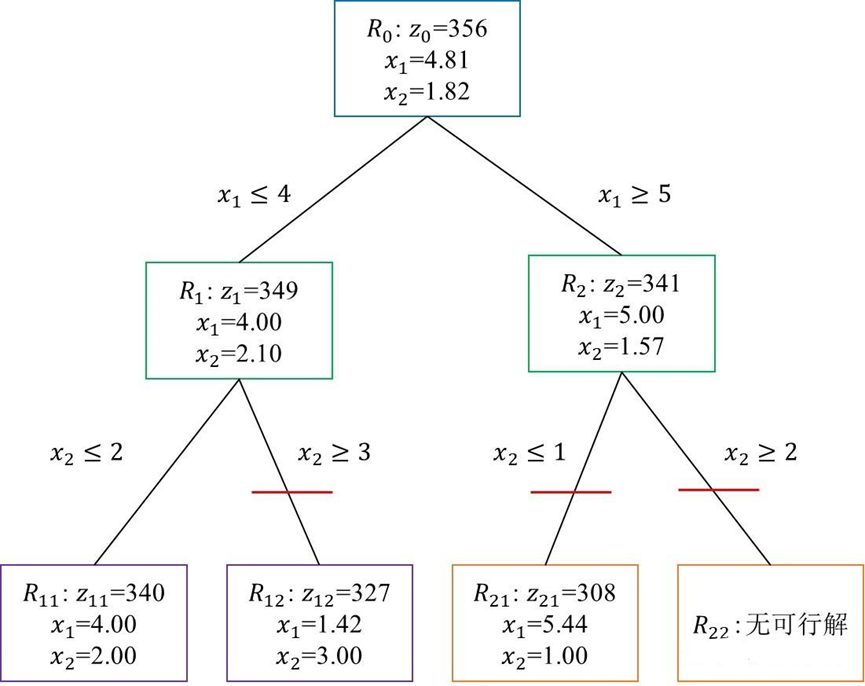
\includegraphics[width=0.5\textwidth]{pic13.png}
    \caption{分支定界法示意图}
    \label{pic13}
\end{figure}

\subsubsection{分支割平面法}
分支割平面法是结合分支定界法和割平面法的一种求解整数线性规划问题的方法。其基本思想是在分支定界法的基础上,通过添加有效的不等式(割平面)来收缩可行解空间,从而更快地找到最优解。

具体步骤如下:
\begin{enumerate}
    \item 求解整数线性规划问题的松弛问题,得到一个下界或上界。
    \item 选择一个非整数解的决策变量,进行分支操作,将问题分解为多个子问题。
    \item 对每个子问题,通过分析其松弛问题的解,寻找有效的不等式(割平面),添加到子问题的约束条件中,进一步缩小可行解空间。
    \item 重复步骤 2 和 3,不断分支和添加割平面,同时记录每个子问题的目标函数值和可行解。
    \item 在分支和割平面的过程中,如果某个子问题的目标函数值超过了已知的最优目标函数值(对于最小化问题)或小于已知的最优目标函数值(对于最大化问题),则剪掉该子问题的分支。
\end{enumerate}

当所有分支都被探索完毕或达到一定的迭代次数时,记录的目标函数值最大的(或最小的)可行解即为整数线性规划问题的最优解。

\subsection{动态规划}
动态规划是一种用于求解多阶段决策问题的优化方法,特别适用于特定类型的整数规划问题,尤其是在离散决策问题中。


动态规划的基本思想是将一个复杂的多阶段决策问题分解为若干个相互关联的子问题,通过求解子问题的最优解,逐步构建出原问题的最优解。其关键在于找到问题的阶段划分、状态转移方程和决策函数。


例如,在背包问题中,有一个背包和若干个物品,每个物品有重量和价值,背包的容量有限,目标是在不超过背包容量的前提下,选择物品使得背包中的物品总价值最大。这个问题可以使用动态规划求解,将问题划分为若干个阶段,每个阶段对应一个物品的决策,状态表示当前背包的剩余容量,决策函数表示是否选择当前物品,通过状态转移方程递推求解最优解。

\subsection{OR-Tools 功能与算法概述}
OR-Tools 是由 Google 开发的一套开源优化工具包,旨在帮助开发者解决各种复杂的组合优化问题。它提供了多种求解器,支持多种编程语言,包括 Python、Java、C++ 和 C\#。OR-Tools 的核心功能包括线性规划、整数规划、约束规划、车辆路径规划和图算法等。

\subsection{OR-Tools 的使用}
OR-Tools的使用主要分为定义决策变量、构建约束条件、定义目标函数、使用求解器进行求解几个步骤,该过程的流程图如图\ref{pic14}所示。

\begin{figure}[h]
    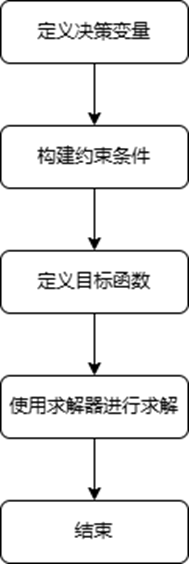
\includegraphics[width=0.3\textwidth]{pic14.png}
    \caption{OR-Tools 使用流程}
    \label{pic14}
\end{figure}

以下是具体的步骤和方法:
\begin{enumerate}
    \item \textbf{定义决策变量}\\
    在使用 OR-Tools 解决问题之前,首先需要明确决策变量。在本问题中,定义整数决策变量 $res_i$,其中$i$代表组件的编号,$res_i$ 表示第$i$个组件的使用数量,且 $res_i \geq 0$。在本问题中,$res_1$可能表示某种特定型号的CPU使用数量,$res_2$ 表示另一种型号的GPU使用数量。这些决策变量是后续构建约束条件和目标函数的基础,准确地定义它们对于问题的求解至关重要。
    
    \item \textbf{构建约束条件}\\
    在明确了决策变量之后,接下来需要构建约束条件。对于每个性能或功能指标 $j$,需要建立线性约束条件:
    \begin{equation}
    c_j \leq \sum_{i=1}^n res_i \cdot a_{i,j} \leq d_j
    \end{equation}
    其中 $a_{i,j}$是第 $i$个组件在指标 $j$上的贡献,$c_j$是对于该指标总和的下限,$d_j$是对于该指标总和的上限(可以为无穷大)。在本问题中,假设性能指标 $j$ 为算力需求,$a_{i,j}$ 表示不同型号芯片对算力的贡献,$c_j$ 和 $d_j$ 分别表示系统所需的最小和最大算力。通过构建这样的约束条件,可以确保所选器件的组合能够满足系统的性能或功能要求。
    
    \item \textbf{定义目标函数}\\
    目标是最小化总成本:
    \begin{equation}
    \sum_{i=1}^n res_i \cdot e_i
    \end{equation}
    其中$e_i$是第 $i$个组件的代价。该代价可以是成本、功耗、面积等,也可以是这些代价组合得到的一个数值。在本问题中,$e_i$ 可以是芯片的成本与功耗的加权和。通过定义目标函数,可以明确优化的方向,即在满足约束条件的前提下,寻找成本最低的组件配置方案。
    
    \item \textbf{使用求解器进行求解}\\
    为了求解上述问题,计划使用开源求解器 OR-Tools。OR-Tools 提供了丰富的接口,可以方便地与 Python 语言进行交互。求解过程主要分为以下几个步骤:
    \begin{enumerate}
        \item \textbf{求解器初始化}\\
        首先,通过 \texttt{solver = pywraplp.Solver.CreateSolver('SCIP')} 指令创建一个求解器。这里选择的求解器是 SCIP,它是一个高性能的混合整数规划求解器。然后,通过 \texttt{x = solver.IntVar(0.0, infinity, 'x')} 指令创建一个整数变量 $x$,并对变量的非负性进行约束。这一步是求解过程的基础,确保了决策变量的合理性和有效性。
        
        \item \textbf{线性约束添加}\\
        在求解器初始化之后,需要添加线性约束。通过 \texttt{constraint0 = solver.Constraint(-solver.infinity(), 14)} 指令可创建一个约束范围,其中 \texttt{-solver.infinity()} 表示约束的下限为负无穷大,14 表示约束的上限。然后,通过 \texttt{constraint0.SetCoefficient(x, 1)} 指令为这个约束范围添加系数。这一步是将之前构建的约束条件具体化,将其转化为求解器可以理解和处理的形式。
        
        \item \textbf{目标函数添加}\\
        在添加了线性约束之后,需要定义目标函数。通过 \texttt{objective = solver.Objective()} 指令可以创建一个目标函数,然后通过一个叫 \texttt{objective.SetCoefficient(x, 3)} 指令为目标函数设置系数。这里的系数 3 表示变量 $x$ 在目标函数中的权重。最后,通过 \texttt{objective . SetMinimization()} 函数设置将目标函数最小化。这一步是明确优化目标的关键步骤,确保求解器能够朝着期望的方向进行优化。
        
        \item \textbf{调用求解器进行求解}\\
        在完成了上述步骤之后,可以调用求解器进行求解。通过 \texttt{status = solver.Solve()} 指令可调用求解器对问题进行求解,并得到求解的状态。状态为 OPTIMAL 表示已找到最优解。这一步是求解过程的核心,求解器将根据之前定义的决策变量、约束条件和目标函数,运用先进的算法寻找最优解。
        
        \item \textbf{输出求解结果}\\
        最后,通过 \texttt{x.solution\_value()} 指令可以得到各个变量的求解结果,并可以通过该结果计算出最优的代价。这一步是求解过程的终点,也是获取最终解决方案的关键步骤。通过输出求解结果,可以明确每个组件的最优使用数量,以及对应的最低成本。
    \end{enumerate}
\end{enumerate}

\section{仿真器的平台搭建}
本节围绕LegoSim异构芯片并行仿真器展开,系统阐述了其设计目标、架构创新、多平台集成能力及验证体系,构建了从大规模异构系统仿真到需求验证的全流程解决方案。该工具链的突破性设计显著提升了仿真效率和可扩展性,为微系统需求定义模型提供精准验证支撑。


\subsection{概述}
LegoSim(用于异构芯片的并行乐高仿真器)旨在应对由异构芯片构建的庞大系统的模拟挑战。

由于主机性能和内存空间的限制,庞大规模的系统无法实现周期精确模型。并行周期精确模型也不具吸引力,因为随着并行程度的提高,所有并行线程或进程之间的同步操作会越来越频繁,速度也无法进一步提高。

传统上,集成一种新的 IP 或芯片是一项艰巨的任务,需要在编码、调试和相关性方面投入大量精力。然而,CPU、NoC、DRAM 等都有开源模型,因此无需从头开始。

对基于芯片的大规模系统进行仿真,仿真速度和开发速度比仿真结果是否与现实系统的周期一致更为重要。学术领域和工业领域都在寻求一种平衡的解决方案。LegoSim 提供了一种松耦合并行架构,以应对更快的仿真、开发和重新配置所带来的挑战。

为加快并行仿真速度,仿真进程之间的同步频率会降低到与基准中的软件同步频率相同。换句话说,只有当基准发送/读取数据或需要共享资源时,仿真进程才会同步。同时,同步范围限制在与软件操作相关的进程。

例如,如果两个模拟进程从不相互通信或从不需要共享资源,那么这两个模拟进程就可以一直并行运行。

再比如,当 CPU 想要向 GPU 发送数据时,CPU 中的软件会将数据写入一定范围的内存空间,并写入另一个内存位置,向 GPU 发出信号,表示数据已准备就绪。在 GPU 读取数据之前,GPU 中的软件会查询内存位置,直到收到信号为止。在 LegoSim 中,这样的操作序列被抽象为一种事务(数据事务)。LegoSim 关注的是一个事务的结束周期,而不是一个事务中每个操作的持续时间。这样,基本同步操作的数量就会减少。


\subsection{目标建模}
芯片仿真器旨在模拟由异构 IP 和芯片组成的系统。

目标架构分为处理组件(PComp)和共享组件(SComp)。一般来说,PComps 是主设备,可生成共享组件请求。PComps 可以选择执行指令,但通常由一个内存系统组成。CPU (集群)、GPU 和 NPU 是典型的 PComps。SComps 由 PComps 共享,并响应来自 PComps 的请求,包括 NoC、DRAM 控制器和某些类型的加速器。

目标架构与芯片组相结合的示例如下:
\begin{figure}[h]
    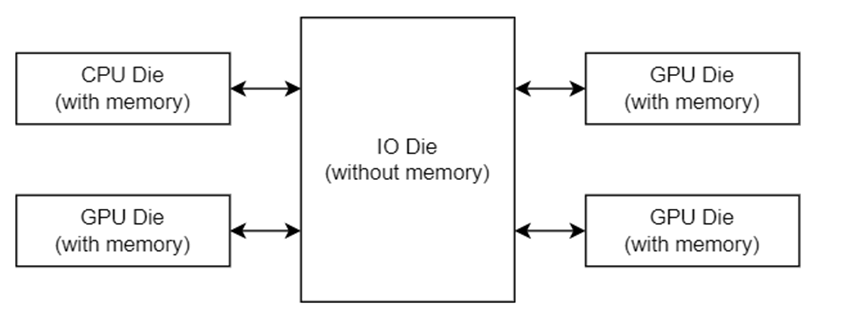
\includegraphics[width=0.7\textwidth]{pic15.png}
    \caption{目标架构与芯片组相结合的示例A}
    \label{pic15}
\end{figure}

下图是目标架构与 IP 结合的另一个例子:
\begin{figure}[h]
    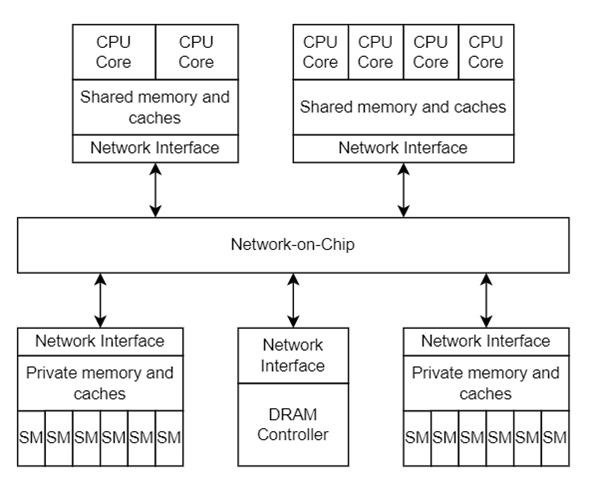
\includegraphics[width=0.5\textwidth]{pic16.png}
    \caption{目标架构与 IP 结合的示例B}
    \label{pic16}
\end{figure}

在执行时间方面,PComps 控制着系统中的任务和流程,在调节模拟时间方面发挥着重要作用。SComps 通过响应 PComps 请求的时间长短来影响性能。以 DRAM 控制器为例,CPU/GPU 会向 DRAM 控制器发送读/写请求。如果 DRAM 访问外部存储器的速度较慢,CPU/GPU 就需要更长的时间来等待 DRAM 控制器的响应,这通常意味着执行一个基准所需的时间更长。因此,如果 SComps 的时间成本能合理地通过 PComps 反映出来,模拟结果将是合理的。


\subsection{LegoSim架构}
如上所述,目标系统由不同类型的组件组合而成,这些组件可由常用的仿真器进行描述。目标系统中的每个组件对应一个仿真进程,这些进程并行执行,以提高仿真速度。

SComp仿真器需要从PComp仿真器获取轨迹作为输入,而PComp仿真器则需要从SComp仿真器获取延迟信息。刺激轨迹和延迟信息都控制着模拟的准确性。因此,LegoSim定义了一个迭代流程,以便PComp和SComp之间的影响能够收敛到一个切合实际的值。

下图显示了迭代流程:
\begin{figure}[h]
    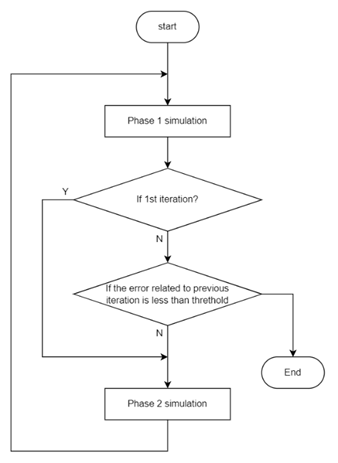
\includegraphics[width=0.5\textwidth]{pic17.png}
    \caption{LegoSim迭代流程}
    \label{pic17}
\end{figure}

每次迭代包括两个阶段。第一阶段模拟PComps,第二阶段模拟SComps。

在第一次迭代的第1阶段,并行模拟PComps。一种算法用于计算PComps请求的延迟。同时,Interchiplet接收来自模拟进程的协议命令,并生成轨迹作为SComps的激励。在第一次迭代中,所有PComps中的最大执行周期被算作该基准的执行周期。

在第一迭代的第二阶段,SComps也是并行模拟的。第1阶段生成的轨迹驱动第2阶段的SComps模拟。仿真会生成每个请求的延迟信息。

在第二次迭代的第1阶段,PComps与第一次迭代一样再次进行模拟。模拟使用上一次迭代第二阶段生成的延迟信息。在第二次迭代的第1阶段结束时,比较当前迭代和前一次迭代记录的执行周期。如果误差比低于指定阈值,则认为执行周期收敛,模拟停止。否则,模拟继续进行第2阶段,与前一次迭代相同。

在不收敛的情况下,模拟流程可以在指定的迭代次数(称为超时)后停止。通过这种迭代收敛机制,LegoSim能够将时序误差控制在1.8\%以内,实现高精度的协同仿真。


\subsection{多进程多线程结构}
LegoSim 是一款多进程、多线程软件。软件结构如下所示:

作为主进程,Interchiplet控制着整个仿真流程。它将创建与仿真进程一样多的线程。这些线程被称为子线程。每个线程对应一个仿真进程,并处理进程间通信和同步。

为避免模拟进程之间的文件冲突,每个迭代进程都有一个单独的文件夹,名为\texttt{proc\_r\{迭代\}\_p\{阶段\}\_t\{线程\}}。例如,\texttt{proc\_r2\_p1\_t4}是第二次迭代第1阶段第4个线程的工作目录。这些文件夹作为子目录被引用。

下图显示了LegoSim的数据流:
\begin{figure}[h]
    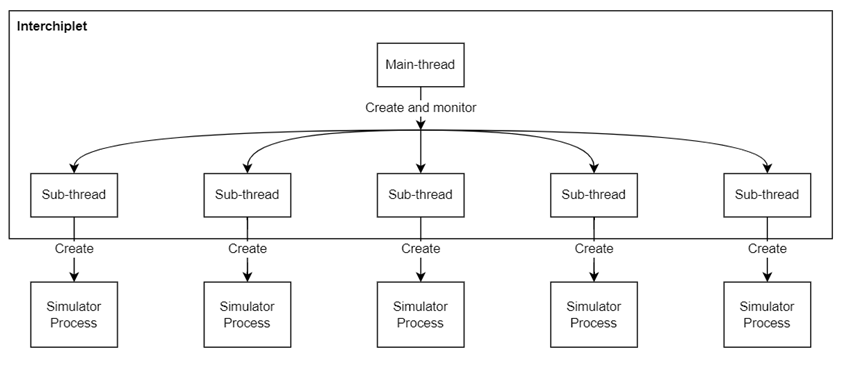
\includegraphics[width=0.7\textwidth]{pic18.png}
    \caption{LegoSim的数据流结构}
    \label{pic18}
\end{figure}

在图\ref{pic18}中,点线表示一个程序内通过变量进行的数据流。粗线表示通过文件描述符(包括管道、命名管道和标准文件接口)进行的数据流。细线表示创建命名管道的控制流。

Interchiplet的每个子线程都通过PIPE连接一个仿真进程的标准输入和输出。标准输出和标准错误输出的内容将重定向到日志文件。

模拟进程之间的数据交换通过命名管道进行。一个命名管道支持单向数据传输。命名管道的创建是必不可少的。LegoSim提供了同步协议和一套应用程序接口(API)来处理进程间的通信。若要在集成的第三方仿真器中应用该协议,只需稍作修改即可。详情请参见同步协议和导入仿真器。

\begin{figure}[h]
    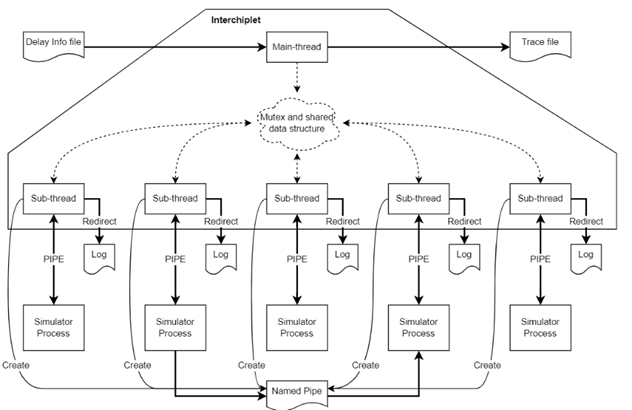
\includegraphics[width=0.3\textwidth]{pic19.png}
    \caption{LegoSim的同步通信机制}
    \label{pic19}
\end{figure}

Interchiplet中的子线程负责处理此类协议。一个子线程通过标准输出从相应的仿真进程获取一条协议命令,并通过标准输入发出另一条协议命令作为响应。

Interchiplet在这些子线程之间维护一个互斥和一个共享数据结构。子线程在处理来自仿真进程的输出时是并行的,因此可以隐藏重定向效果。当它们收到任何协议命令时,其中一个线程必须在进一步处理之前锁定互斥,因此所有协议命令都是原子处理的。

在创建子线程之前,Interchiplet的主线程会将上一迭代阶段2生成的延迟信息加载到共享数据结构中。所有子线程都能通过共享数据结构获取包延迟信息。子线程在仿真过程中接收协议命令,并在共享数据结构中记录跟踪信息。所有子线程结束后,Interchiplet的主线程将把共享数据结构中记录的轨迹转存到文件中,作为第2阶段的激励。


\section{NEMU的模拟器搭建}
\subsection{NEMU概述}
NEMU(NJU EMUlator)是一个轻量级的计算机系统模拟器,最初由南京大学开发用于教学目的,现已发展成为一个强大的CPU模拟平台。在芯粒设计自动化流程中,NEMU作为预仿真工具发挥着至关重要的作用,能够在详细仿真前提供快速的功能验证和性能评估。

与LegoSim等大型异构仿真平台相比,NEMU具有启动速度快、资源占用少、配置灵活等特点,特别适合在芯片设计早期阶段进行快速原型验证和算法测试。NEMU支持多种指令集架构(ISA),包括x86、RISC-V、ARM等,这使其成为异构芯粒设计中不可或缺的工具。

\subsection{NEMU架构设计}
NEMU采用模块化架构设计,主要由指令译码器、功能单元模拟器、存储层次模拟器、设备模拟器和调试接口等核心组件构成。其总体架构如图\ref{pic20}所示:

\begin{figure}[h]
    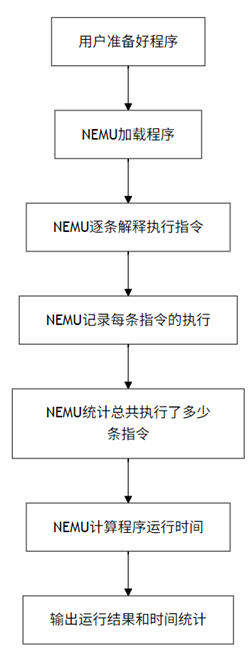
\includegraphics[width=0.3\textwidth]{pic20.png}
    \caption{NEMU模拟器架构}
    \label{pic20}
\end{figure}

主要组件功能如下:
\begin{enumerate}
    \item \textbf{指令译码器}:负责将机器指令解码为可执行的微操作,支持多种指令集架构。
    \item \textbf{功能单元模拟器}:模拟CPU各功能单元的行为,包括算术逻辑单元、浮点运算单元等。
    \item \textbf{存储层次模拟器}:模拟从寄存器到主存的完整存储层次,支持缓存一致性协议。
    \item \textbf{设备模拟器}:提供基本I/O设备的模拟,如串口、时钟等。
    \item \textbf{调试接口}:提供丰富的调试功能,支持断点、单步执行、寄存器/内存检查等。
\end{enumerate}

NEMU采用解释执行方式模拟指令执行,通过查询指令译码表将每条指令映射到对应的处理函数,实现指令的功能模拟。这种设计使NEMU在保持高灵活性的同时,也能提供足够的模拟精度。

\subsection{NEMU的模拟流程}
NEMU模拟器的基本工作流程包括初始化、取指、译码、执行和调试等阶段,如图\ref{pic21}所示:

\begin{figure}[h]
    \makebox[\textwidth][c]{\includegraphics[width=2.0\textwidth]{pic21.png}}
    \caption{NEMU基本工作流程}
    \label{pic21}
\end{figure}

具体流程说明如下:
\begin{enumerate}
    \item \textbf{初始化阶段}:加载配置参数,初始化虚拟机状态,包括寄存器组、内存空间和设备状态。
    \item \textbf{程序加载}:将待执行的程序二进制文件加载到模拟器的虚拟内存空间。
    \item \textbf{指令执行循环}:
    \begin{itemize}
        \item \textbf{取指}:从PC(程序计数器)指向的内存位置获取指令。
        \item \textbf{译码}:将机器码指令解析为具体的操作码和操作数。
        \item \textbf{执行}:调用对应的指令处理函数,模拟指令执行过程。
        \item \textbf{更新状态}:更新寄存器值、内存内容和设备状态。
    \end{itemize}
    \item \textbf{调试交互}:在需要时进入调试模式,支持用户交互操作。
    \item \textbf{结果输出}:执行完成后,输出执行统计信息、性能指标等。
\end{enumerate}

NEMU支持两种主要的模拟模式:
\begin{itemize}
    \item \textbf{功能模拟模式}:仅模拟指令的功能效果,不考虑硬件时序,执行速度快。
    \item \textbf{时序模拟模式}:考虑流水线、缓存等微架构特性的影响,提供更准确的性能估计。
\end{itemize}

\subsection{NEMU在芯粒设计中的应用}
在芯粒设计自动化流程中,NEMU主要用于以下几个方面:

\begin{enumerate}
    \item \textbf{功能验证}:在详细的系统级仿真前,使用NEMU验证芯粒设计的基本功能正确性,节省设计周期。
    \item \textbf{性能评估}:通过内置的性能计数器,对设计方案进行初步性能评估,指导优化方向。
    \item \textbf{软件开发}:为应用开发人员提供快速的软件开发和测试环境,加速软硬件协同设计。
    \item \textbf{接口验证}:验证芯粒间的通信接口和协议设计,确保系统级集成的可行性。
\end{enumerate}

相比LegoSim等复杂的异构仿真平台,NEMU作为预仿真工具具有以下优势:
\begin{itemize}
    \item \textbf{速度优势}:NEMU的功能模拟模式比周期精确模拟快1-2个数量级,适合快速迭代设计。
    \item \textbf{资源高效}:占用计算资源少,可在普通工作站上运行复杂模拟。
    \item \textbf{易于配置}:配置简单,启动迅速,适合频繁的设计空间探索。
    \item \textbf{调试友好}:提供丰富的调试工具和接口,便于定位和解决问题。
\end{itemize}

\subsection{NEMU的搭建与配置}
NEMU模拟器的搭建过程主要包括环境准备、源码获取、编译配置和运行测试四个步骤,具体如下:

\begin{enumerate}
    \item \textbf{环境准备}:
    \begin{itemize}
        \item 安装必要的开发工具:gcc, make, autoconf等。
        \item 安装依赖库:readline, SDL2, libdisasm等。
    \end{itemize}

    \item \textbf{源码获取与编译}:
    \begin{verbatim}
git clone https://github.com/NJU-ProjectN/nemu.git
cd nemu
make menuconfig  # 配置模拟器参数
make
    \end{verbatim}

    \item \textbf{模拟器配置}:
    \begin{itemize}
        \item 选择目标指令集架构(x86, RISC-V, ARM)
        \item 配置存储层次参数(缓存大小、相联度等)
        \item 设置调试选项和性能监测点
    \end{itemize}

    \item \textbf{运行与测试}:
    \begin{verbatim}
./build/nemu -l [log_file] -b [benchmark] -d [device_config]
    \end{verbatim}
\end{enumerate}

在芯粒设计自动化流程中,NEMU通常结合配置脚本使用,以自动化执行不同设计方案的模拟和比较。这些脚本可以控制模拟参数,收集性能数据,并生成比较报告,为设计决策提供依据。

\subsection{NEMU与协同仿真的集成}
为实现全面的异构芯粒设计验证,NEMU可以与LegoSim等系统级仿真平台集成,形成完整的仿真工具链。集成方式主要有以下几种:

\begin{enumerate}
    \item \textbf{松耦合集成}:NEMU作为独立的预仿真工具,其结果作为LegoSim等详细仿真的输入,提供初始估计和优化方向。

    \item \textbf{API级集成}:通过定义统一的接口,将NEMU作为一个模块集成到LegoSim框架中,实现数据共享和协同仿真。

    \item \textbf{工作流集成}:在设计自动化工作流中,NEMU和LegoSim作为不同阶段的工具,由工作流管理工具协调运行。
\end{enumerate}

通过这种分层集成的方式,可以充分发挥NEMU快速预仿真和LegoSim精确系统仿真的各自优势,提高整体设计效率和质量。

\subsection{小结}
NEMU作为一个轻量级但功能强大的CPU模拟器,在芯粒设计自动化流程中发挥着重要的预仿真作用。它通过快速的功能验证和初步性能评估,为后续的详细仿真提供有效指导,显著缩短设计周期。与LegoSim等系统级仿真工具相结合,形成了从快速预仿真到精确系统仿真的完整工具链,为异构芯粒设计自动化提供了有力支持。

在未来工作中,可考虑进一步增强NEMU的指令级并行建模能力,优化其与系统级仿真工具的集成接口,以及扩展对新型指令集架构和专用加速器的支持,以适应不断发展的异构集成芯片设计需求。

\section{总结}

本章系统性地阐述了芯粒设计自动化的基础理论与关键技术,为后续的设计实现奠定了坚实基础。主要内容可概括为以下几个方面:

首先,从需求定义角度入手,分析了集成电路技术发展的主要趋势及其对芯粒需求的影响,包括尺寸缩小与性能提升、能效优化、多核与异构计算以及物联网智能化等方向。通过对比瀑布模型、敏捷模型、V模型、螺旋模型和迭代增量模型等现有需求定义模型的优缺点,提出了适用于芯粒设计的复合需求定义模型,实现了从系统需求到元器件选型的精确映射。

然后,深入研究了线性规划在芯粒选型过程中的理论基础与应用方法,详细阐述了目标函数的构建、约束条件的设定以及各种求解方法,包括图解法、单纯形法、对偶单纯形法和分支定界法等。特别是介绍了基于OR-Tools的线性规划求解框架,为芯粒在功耗、成本等多目标约束下的器件选型优化提供了有效工具。

然后,系统性地探讨了LegoSim异构仿真平台的架构设计与工作流程,分析了其多进程多线程的软件结构、目标建模方法和迭代收敛机制,揭示了如何通过松耦合并行架构实现高效的异构芯片仿真,有效控制时序误差在1.8\%以内。

最后,详细介绍了NEMU轻量级CPU模拟器的架构设计、模拟流程和应用优势。作为预仿真工具,NEMU在芯粒设计自动化流程中扮演着快速功能验证和性能评估的重要角色,与LegoSim等系统级仿真平台形成了互补关系,构建了从快速预仿真到精确系统仿真的完整工具链。

通过以上基础研究,本章建立了从需求定义、器件选型到仿真验证的系统化方法论,为芯粒设计自动化提供了理论指导和技术支撑。这些方法和工具的有机结合,为下一章中基于芯粒库的设计自动化方法的具体实现创造了有利条件。





\chapter{芯粒设计自动化的实现}

\section{芯粒设计自动化的总体框架}

芯粒设计自动化框架主要由四个核心环节组成:基于NEMU的预仿真、基准测试选择、基于整数线性规划的芯粒选型以及基于LegoSim的系统级仿真验证。这四个环节形成闭环设计流程,通过迭代优化提升设计质量。如图\ref{fig:framework}所示,整个框架采用自顶向下的设计方法,支持从系统需求到具体实现的全流程设计。

\begin{figure}[htbp]
    \makebox[\textwidth][c]{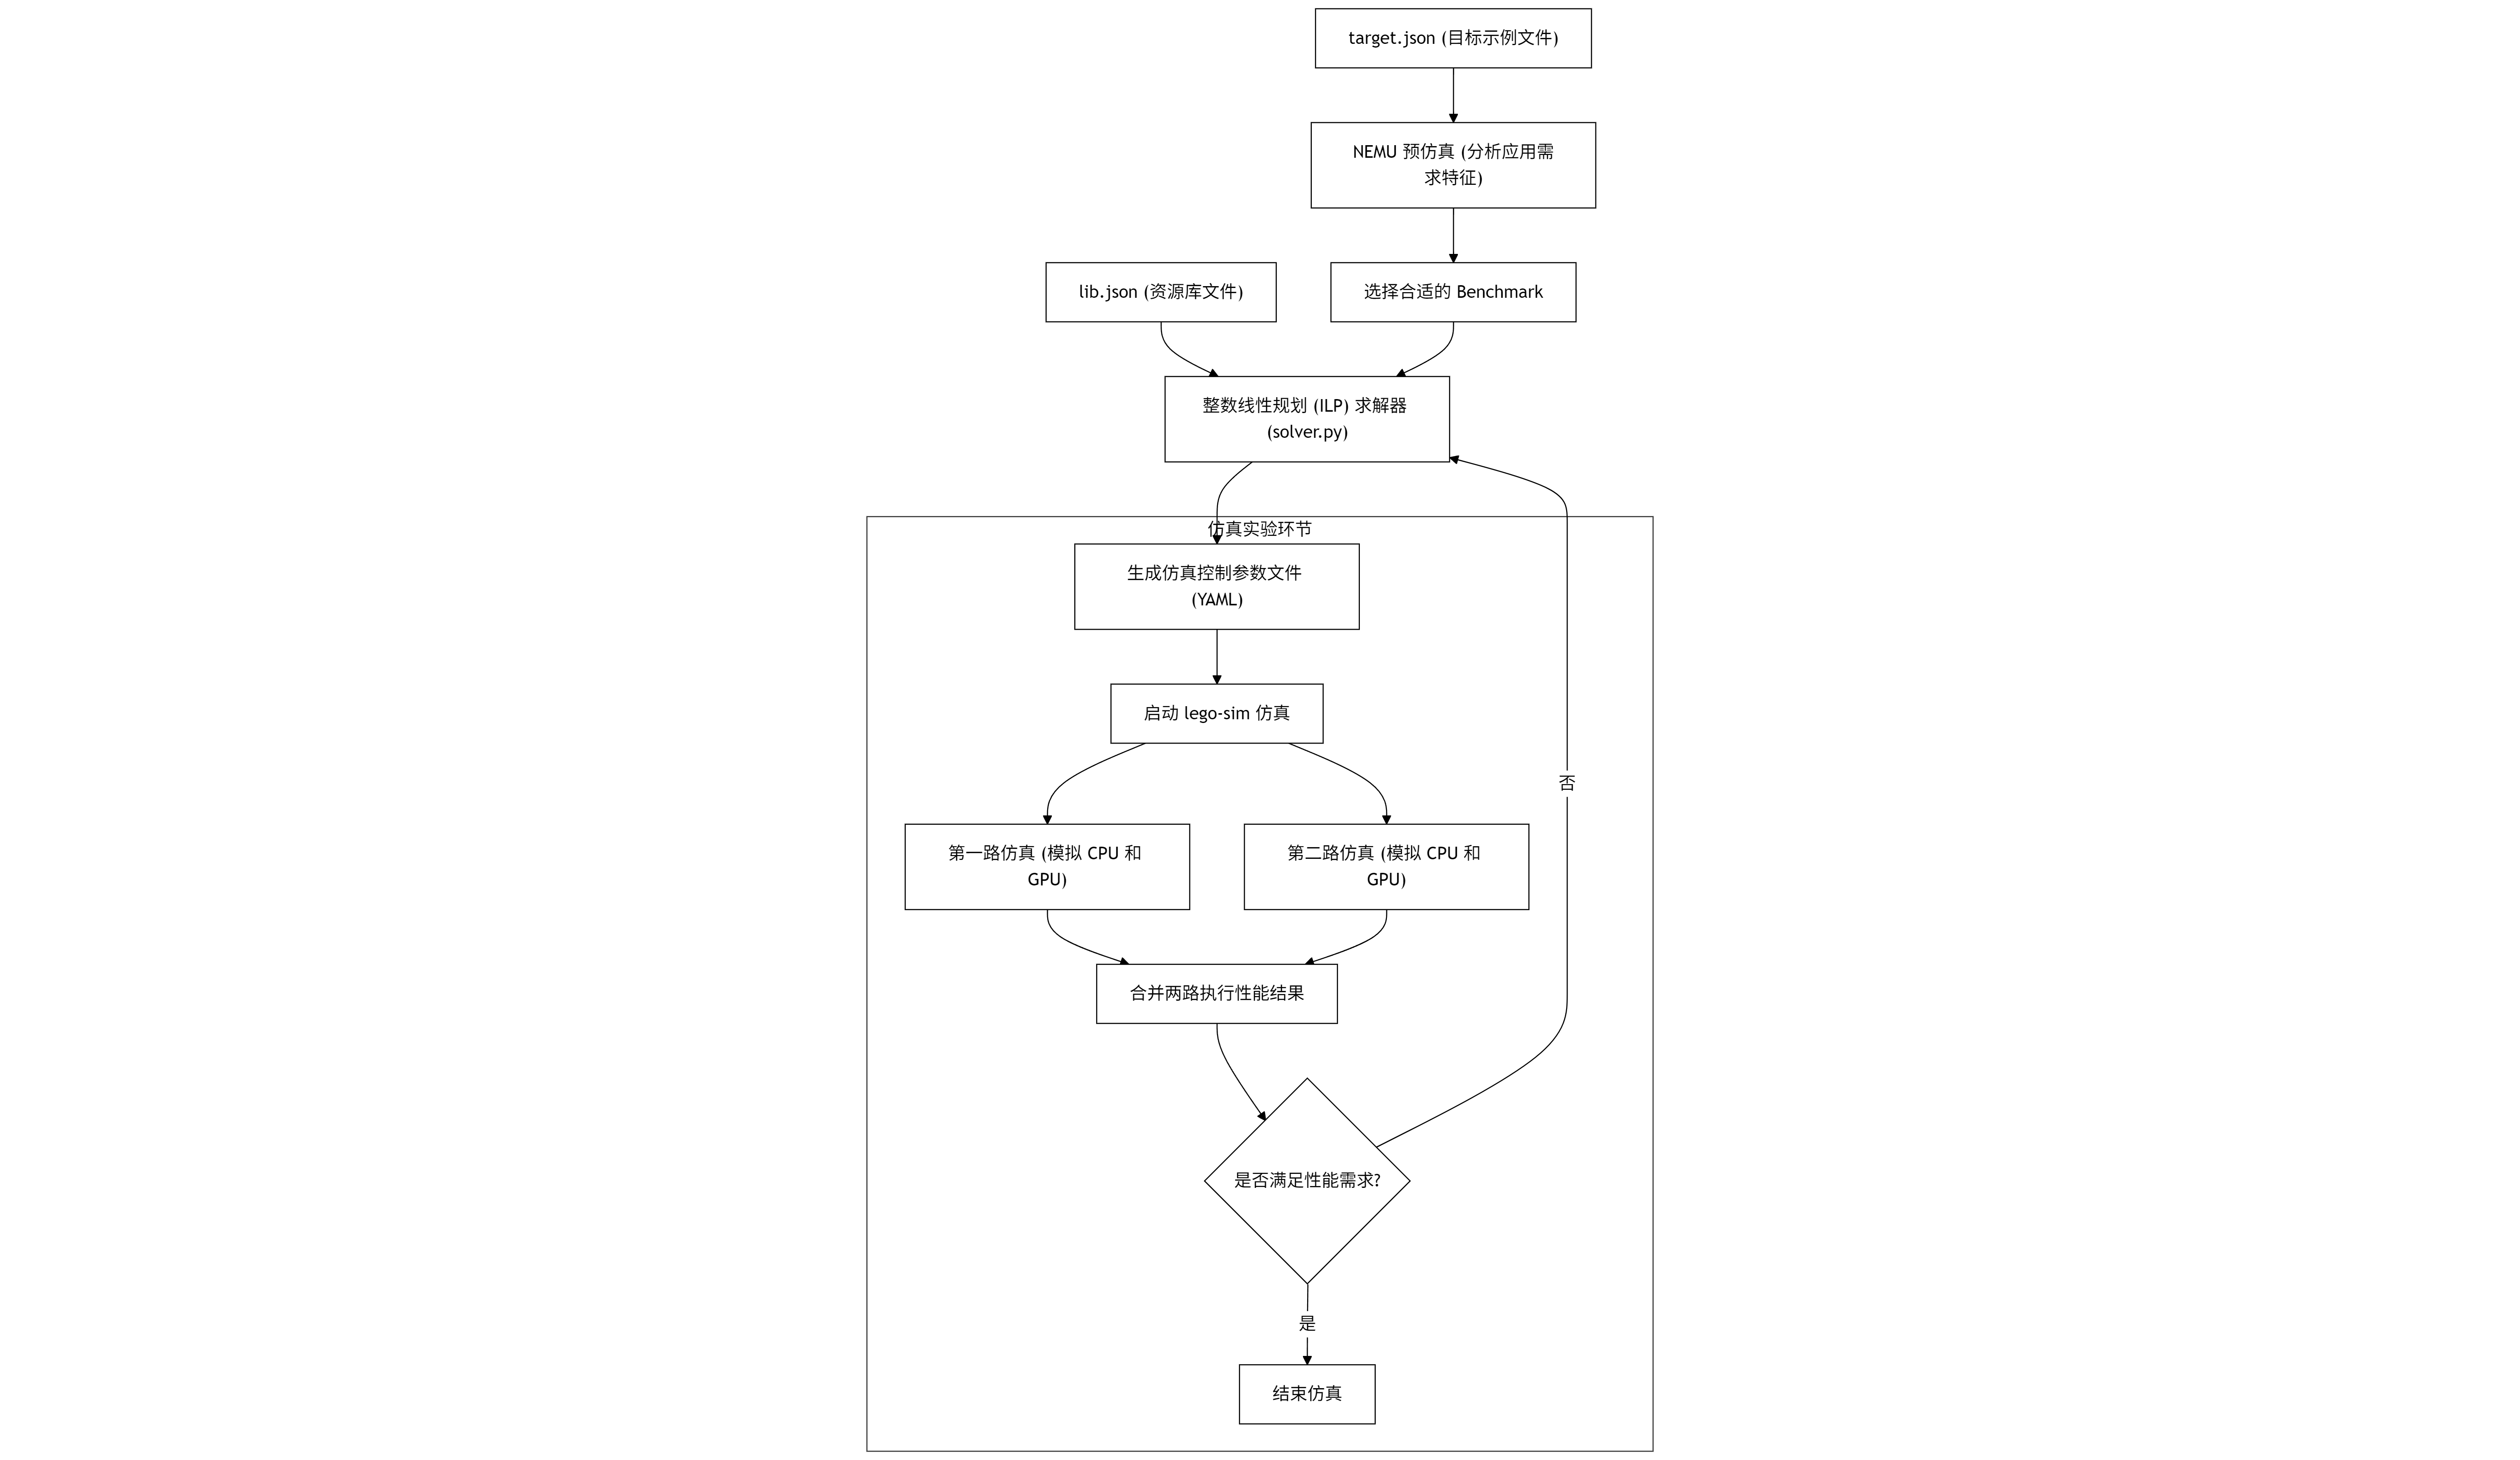
\includegraphics[width=1.4\textwidth]{芯粒设计自动化的总体框架.png}}
    \caption{芯粒设计自动化总体框架}
    \label{fig:framework}
\end{figure}

此框架的主要优势在于:
\begin{itemize}
    \item \textbf{自动化程度高}:降低设计复杂性和出错风险
    \item \textbf{设计效率高}:通过预仿真和自动优化提高设计效率
    \item \textbf{设计空间广泛}:在广泛设计空间中寻找最优解
    \item \textbf{多目标优化}:同时考虑性能、功耗、成本等多个目标
    \item \textbf{精确验证}:提供全面的系统级仿真验证手段
\end{itemize}

\subsection{芯粒库设计与实现}

芯粒库是整个设计自动化框架的基础,提供了预制芯粒组件供设计过程选择。如图\ref{fig:chiplet_lib}所示,芯粒库采用分层结构组织,包含各类组件的详细参数和特性。

\begin{figure}[htbp]
    \centering
    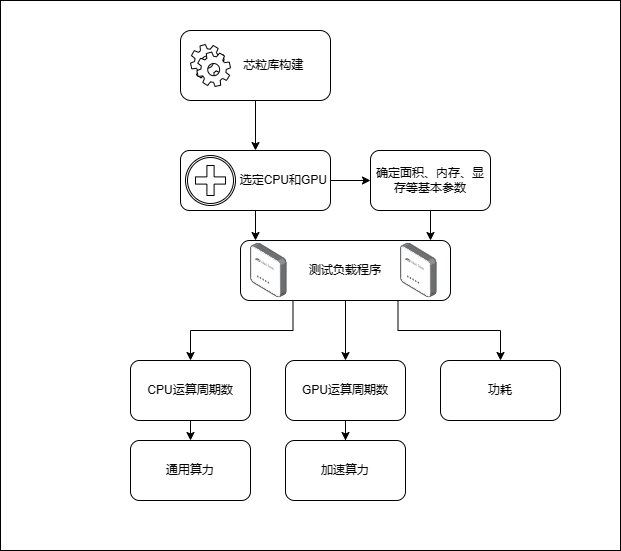
\includegraphics[width=0.8\textwidth]{芯粒库的构建.png}
    \caption{芯粒库的结构与组织}
    \label{fig:chiplet_lib}
\end{figure}

芯粒库根据功能类型分为以下几个主要类别:

\begin{enumerate}
    \item \textbf{处理芯粒}:不同性能等级的CPU、GPU、AI加速器等
    \item \textbf{存储芯粒}:各类缓存控制器、内存控制器等
    \item \textbf{互连芯粒}:NoC路由器、高速接口、总线接口等
    \item \textbf{辅助芯粒}:电源管理、时钟控制、安全模块等
\end{enumerate}

芯粒库中的每个条目包含标识信息、功能属性、性能参数、物理特性、经济指标、可靠性数据和接口规范等属性。

\begin{table}[htbp]
\caption{芯粒库中不同类型组件的关键参数}
\centering
\begin{tabular}{|p{2.5cm}|p{2.5cm}|p{2.5cm}|p{2.5cm}|p{2.5cm}|}
\hline
\textbf{参数类别} & \textbf{处理芯粒} & \textbf{存储芯粒} & \textbf{互连芯粒} & \textbf{辅助芯粒} \\
\hline
计算能力 & GOPS/FLOPS & - & - & - \\
\hline
存储容量 & 缓存大小 & 容量(MB/GB) & 缓冲区大小 & - \\
\hline
访问带宽 & 内存带宽 & 读/写速率 & 数据传输速率 & - \\
\hline
功耗 & 静态/动态功耗 & 静态/动态功耗 & 每比特功耗 & 功耗效率 \\
\hline
面积 & 核心面积($mm^2$) & 单位面积($/MB$) & 接口面积 & 控制电路面积 \\
\hline
延迟 & 指令周期 & 访问延迟 & 传输延迟 & 响应时间 \\
\hline
工艺节点 & nm & nm & nm & nm \\
\hline
\end{tabular}
\label{tab:chiplet_params}
\end{table}

\subsection{设计流程管理}

整个框架通过设计流程管理系统进行集成和协调,包括工作流引擎、参数管理、版本控制、结果分析和知识库等组件,支持自动模式和交互模式两种工作方式。

设计流程管理的数学模型可表示为有向无环图(DAG) $G = (V, E)$,其中:
\begin{itemize}
    \item $V = \{v_1, v_2, ..., v_n\}$ 表示设计流程中的各个任务节点
    \item $E = \{e_{ij} | v_i, v_j \in V\}$ 表示任务之间的依赖关系
    \item 每个节点 $v_i$ 具有权重 $w_i$,表示执行该任务所需的时间或资源
\end{itemize}

设计流程的关键路径长度为:
\begin{equation}
CP(G) = \max_{p \in \text{所有路径}} \sum_{v_i \in p} w_i
\end{equation}

通过优化任务依赖关系和资源分配,可以降低关键路径长度,提高设计效率。

\section{基于NEMU的预仿真}

预仿真是芯粒设计自动化流程中的第一个关键环节,旨在快速评估应用特性和性能需求,为后续设计决策提供依据。

\subsection{预仿真的目标与价值}

在芯粒设计自动化流程中,预仿真具有以下几个重要目标:

\begin{enumerate}
    \item \textbf{快速功能验证}:在详细设计前验证基本功能正确性
    \item \textbf{性能特征提取}:分析应用的计算特征和资源需求
    \item \textbf{瓶颈预测}:提前识别潜在的系统瓶颈
    \item \textbf{设计参数估计}:为后续设计阶段提供初步参数
    \item \textbf{设计空间缩减}:缩小后续详细探索的设计空间范围
\end{enumerate}

\subsection{NEMU预仿真流程与周期数估计方法}

本研究采用NEMU(南京大学模拟器)作为预仿真平台,其优势在于启动速度快、资源占用少、配置灵活。NEMU预仿真流程包括准备工作负载、配置环境、运行预仿真、分析性能数据和建立性能模型等步骤。

将benchmark在NEMU中运行后,通过指令分类统计、基本周期成本分配、微架构效应建模、并行度分析和综合周期估计,将执行特性映射到LegoSim中的周期数估计。周期数估计的核心公式如下:

\begin{equation}
Cycles_{LegoSim} = \sum_{i \in InstrTypes} (Count_i \times BaseCost_i \times MicroarchFactor_i) / ParallelismFactor
\end{equation}

为了更精确地估计不同类型指令的执行周期,我们引入了更详细的估计模型:

\begin{equation}
Cycles_{LegoSim} = \alpha \cdot \left( \sum_{i \in ALU} C_i \cdot W_i + \beta \cdot \sum_{j \in MEM} C_j \cdot W_j \cdot M_j + \gamma \cdot \sum_{k \in BRANCH} C_k \cdot W_k \cdot B_k \right)
\end{equation}

其中:
\begin{itemize}
    \item $\alpha$ 是架构相关的调整系数
    \item $C_i$, $C_j$, $C_k$ 分别是ALU指令、访存指令和分支指令的执行次数
    \item $W_i$, $W_j$, $W_k$ 分别是各类指令的基础权重
    \item $M_j$ 是内存访问模式影响因子,与缓存命中率相关:
    $M_j = 1 + (1-h_L1) \cdot p_L1 + (1-h_L2) \cdot p_L2$
    \item $B_k$ 是分支预测影响因子:$B_k = 1 + m_r \cdot p_b$
    \item $\beta$, $\gamma$ 是访存和分支指令的权重系数
    \item $h_L1$, $h_L2$ 是L1、L2缓存命中率
    \item $p_L1$, $p_L2$ 是缓存未命中惩罚
    \item $m_r$ 是分支预测失误率
    \item $p_b$ 是分支预测失误惩罚
\end{itemize}

\begin{table}[htbp]
\caption{不同指令类型的基础周期成本与调整因子}
\centering
\begin{tabular}{|l|c|c|c|c|}
\hline
\textbf{指令类型} & \textbf{基础成本} & \textbf{微架构因子范围} & \textbf{并行度因子} & \textbf{调整系数} \\
\hline
整数运算(ALU) & 1 & 0.8 - 1.2 & 0.25 - 1.0 & $\alpha = 1.0$ \\
\hline
浮点运算(FPU) & 3 - 5 & 0.9 - 1.5 & 0.25 - 1.0 & $\alpha = 1.2$ \\
\hline
载入(Load) & 2 - 4 & 1.0 - 3.0 & 0.5 - 1.0 & $\beta = 1.5$ \\
\hline
存储(Store) & 2 - 3 & 1.0 - 2.5 & 0.5 - 1.0 & $\beta = 1.3$ \\
\hline
条件分支 & 1 - 2 & 1.0 - 5.0 & 0.8 - 1.0 & $\gamma = 2.0$ \\
\hline
函数调用/返回 & 3 - 6 & 1.2 - 2.0 & 1.0 & $\gamma = 1.8$ \\
\hline
SIMD向量运算 & 2 - 8 & 0.5 - 1.0 & 0.1 - 0.25 & $\alpha = 0.8$ \\
\hline
\end{tabular}
\label{tab:instr_costs}
\end{table}

\subsection{指令类型周期成本与调整因子参数设计原理}

表格\ref{tab:instr_costs}中的参数设置是基于现代处理器微架构特性和指令执行模式的深入分析,每个参数的设置都有其特定的性能考量:

\subsubsection{基础成本差异的原理}

\begin{enumerate}
    \item \textbf{整数运算(ALU)} 被设为最低值(1),这是因为整数运算单元通常是处理器中最基础且流水线最深的单元,执行延迟最短。
    
    \item \textbf{浮点运算(FPU)} 的基础成本(3-5)明显高于整数运算,反映了浮点运算在硬件实现上的额外复杂性,包括符号处理、指数和尾数运算等。
    
    \item \textbf{载入(Load)指令} (2-4)比存储(Store)(2-3)略高,这反映了现代CPU中载入指令可能触发的额外操作,如缓存检查、预取队列处理等。
    
    \item \textbf{SIMD向量运算} 虽然单条指令包含多个运算,但基础成本(2-8)体现了向量单元通常设计为高吞吐量而非低延迟。
\end{enumerate}

\subsubsection{微架构因子范围的合理性}

\begin{enumerate}
    \item \textbf{分支指令} 的微架构因子范围最大(1.0-5.0),这体现了分支预测失败带来的极大性能惩罚(管道刷新、上下文恢复等)。
    
    \item \textbf{载入指令} 的范围(1.0-3.0)较大,反映了缓存命中/缺失带来的巨大延迟差异。
    
    \item \textbf{SIMD指令} 的微架构因子可低至0.5,体现了向量指令在理想情况下的超标量执行能力。
\end{enumerate}

\subsubsection{并行度因子的设计考量}

\begin{enumerate}
    \item \textbf{SIMD向量运算} 的并行度因子最低(0.1-0.25),表明单条向量指令可替代多条标量指令,实现高度并行。
    
    \item \textbf{分支和函数调用} 的并行度因子接近1.0,表明这类控制流指令难以并行执行,几乎总是串行的。
    
    \item \textbf{ALU和FPU指令} 的并行度因子较低,反映了现代处理器能同时执行多条算术指令的能力。
\end{enumerate}

\subsubsection{调整系数的整体平衡}

\begin{enumerate}
    \item \textbf{分支指令} 的调整系数最高($\gamma = 2.0$),强调了控制流对性能的关键影响。
    
    \item \textbf{访存指令} 的调整系数较高($\beta = 1.3-1.5$),体现了内存访问通常是性能瓶颈。
    
    \item \textbf{向量指令} 的调整系数较低($\alpha = 0.8$),反映了向量化带来的整体性能提升。
\end{enumerate}

这些参数设置的综合目标是建立一个平衡精确性和复杂性的性能模型,能够在预仿真阶段准确估计不同工作负载在目标芯粒上的执行周期,为后续的芯粒选型优化提供可靠依据。

\subsection{关键性能指标提取}

NEMU还支持提取以下关键性能指标:

\begin{itemize}
    \item \textbf{计算密度}:每字节内存访问对应的计算操作数量
    \begin{equation}
    ComputeDensity = \frac{TotalArithmeticInstructions}{TotalMemoryAccessBytes}
    \end{equation}
    
    \item \textbf{内存访问模式}:顺序访问比例、局部性强度
    \begin{equation}
    TemporalLocality = \frac{CacheHits}{TotalMemoryAccesses}
    \end{equation}
    
    \begin{equation}
    SpatialLocality = \frac{SequentialAccessCount}{TotalMemoryAccessCount}
    \end{equation}
    
    \item \textbf{分支行为}:分支预测难度、控制流复杂度
    \begin{equation}
    BranchEntropy = -\sum_{i=1}^{n} p_i \log_2 p_i
    \end{equation}
    其中$p_i$是第$i$个分支目标的概率
    
    \item \textbf{并行潜力}:指令级、数据级、线程级并行度评估
    \begin{equation}
    ILP = \frac{TotalInstructions}{CriticalPathLength}
    \end{equation}
    
    \item \textbf{功能单元需求}:不同功能单元的使用强度
\end{itemize}

\subsection{针对异构芯粒的性能映射}

为支持异构芯粒性能估计,建立了从NEMU执行特性到不同类型芯粒性能的映射模型,包括CPU芯粒性能映射、GPU芯粒性能映射、专用加速器映射和混合系统映射。

对于CPU芯粒,性能映射模型为:
\begin{equation}
T_{CPU\_Target} = T_{CPU\_NEMU} \times \frac{F_{NEMU}}{F_{Target}} \times \frac{CPI_{Target}}{CPI_{NEMU}} \times \frac{IC_{Target}}{IC_{NEMU}}
\end{equation}

其中:
\begin{itemize}
    \item $T_{CPU\_Target}$ - 目标CPU上的执行时间
    \item $T_{CPU\_NEMU}$ - NEMU上的执行时间
    \item $F_{NEMU}$, $F_{Target}$ - NEMU和目标CPU的时钟频率
    \item $CPI_{NEMU}$, $CPI_{Target}$ - 每指令周期数
    \item $IC_{NEMU}$, $IC_{Target}$ - 指令计数
\end{itemize}

对于GPU芯粒,性能映射模型考虑并行度和数据传输开销:
\begin{equation}
T_{GPU} = T_{comp} + T_{mem} = \frac{OpsCount}{ParallelFactor \times PeakOps} + \frac{DataSize}{MemBandwidth}
\end{equation}

对于异构系统,考虑负载分布和同步开销:
\begin{equation}
T_{hybrid} = mix(T_{CPU}, T_{GPU}) + T_{sync} + T_{comm}
\end{equation}

\begin{table}[htbp]
\caption{性能映射模型的准确性评估}
\centering
\begin{tabular}{|l|c|c|c|c|}
\hline
\textbf{测试用例} & \textbf{实际周期数} & \textbf{估计周期数} & \textbf{相对误差}   \\
\hline
并行矩阵运算 (64×64) & 256,3241 & 278,5902 & 8.6\%  \\
\hline
多层感知器 (MLP) & 427,8567 & 386,1243 & -9.8\%  \\
\hline
\textbf{平均误差} & - & - & 9.2\%  \\
\hline
\end{tabular}
\label{tab:performance_mapping}
\end{table}

通过基准测试集验证、回归分析、误差分析与修正等方法,将NEMU预仿真的周期数估计误差控制在15\%以内。

\section{基准测试选择}

本节介绍为验证芯粒设计自动化方法而实现的两个典型基准测试:并行矩阵运算和多层感知器(MLP)。

\subsection{基准测试选择原则}

本研究在选择和实现基准测试时遵循代表性、可扩展性、可移植性、可分析性和全面覆盖等原则。可以用以下评分模型来评估基准测试的适合度:

\begin{equation}
S_{benchmark} = w_1 \cdot R + w_2 \cdot S + w_3 \cdot P + w_4 \cdot A + w_5 \cdot C
\end{equation}

其中:
\begin{itemize}
    \item $R$ - 代表性分数(0-10)
    \item $S$ - 可扩展性分数(0-10)
    \item $P$ - 可移植性分数(0-10)
    \item $A$ - 可分析性分数(0-10)
    \item $C$ - 覆盖度分数(0-10)
    \item $w_1, w_2, w_3, w_4, w_5$ - 权重系数,满足$\sum_{i=1}^{5} w_i = 1$
\end{itemize}

\begin{table}[htbp]
\caption{目前提供的基准测试的评分对比}
\centering
\begin{tabular}{|l|c|c|c|c|c|c|}
\hline
\textbf{基准测试} & \textbf{代表性} & \textbf{可扩展性} & \textbf{可移植性} & \textbf{可分析性} & \textbf{覆盖度} & \textbf{总分} \\
\hline
并行矩阵运算 & 9 & 10 & 9 & 9 & 8 & 9.0 \\
\hline
多层感知器(MLP) & 10 & 9 & 8 & 8 & 10 & 9.0 \\
\hline
SPEC CPU & 8 & 6 & 7 & 7 & 9 & 7.4 \\
\hline
\end{tabular}
\label{tab:benchmark_scores}
\end{table}

\subsection{并行矩阵运算基准测试}

并行矩阵运算是测试异构芯粒计算能力的理想基准,实现了矩阵乘法、加法、转置和求逆等操作,支持不同的并行计算模型。

\begin{figure}[htbp]
    \centering
    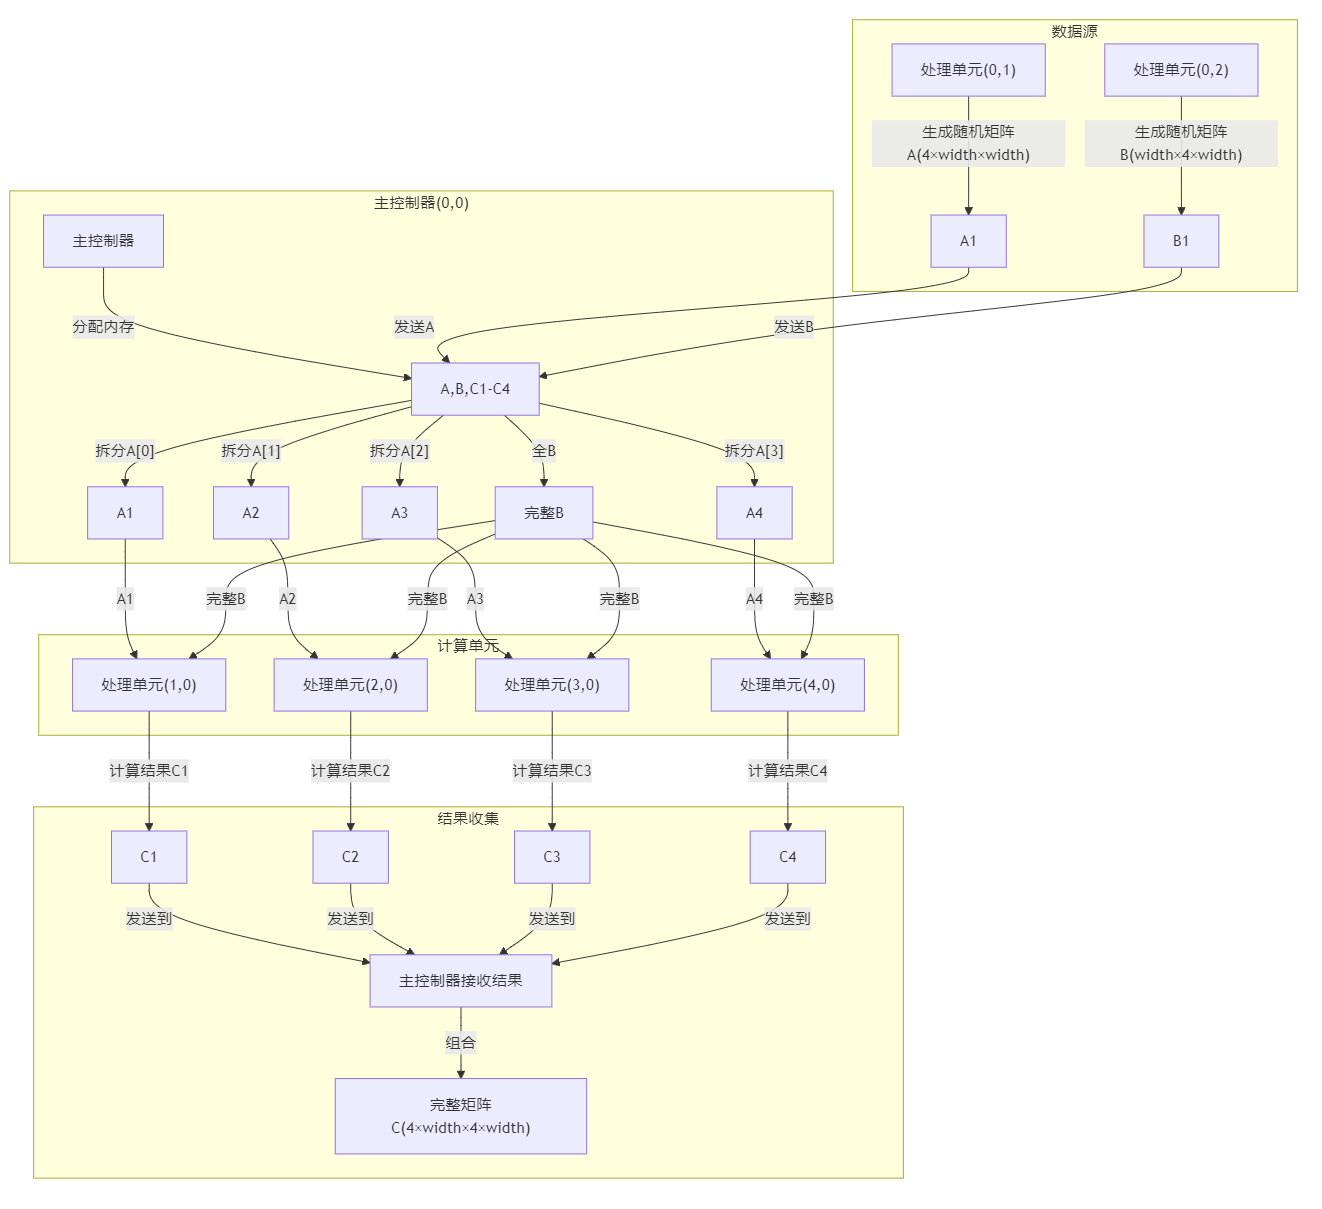
\includegraphics[width=0.8\textwidth]{并行矩阵运算介绍.png}
    \caption{并行矩阵运算基准测试结构与流程}
    \label{fig:matrix_benchmark}
\end{figure}

如图\ref{fig:matrix_benchmark}所示,并行矩阵运算基准测试具有以下主要特点:

\begin{itemize}
    \item \textbf{多种矩阵运算算法}:经典算法、分块算法等
    \item \textbf{可配置的矩阵特性}:维度、数据类型、特殊结构
    \item \textbf{性能分析指标}:计算吞吐量、带宽利用率、并行效率等
\end{itemize}

对于矩阵乘法计算,理论计算量和内存访问量为:

\begin{equation}
\text{FLOP Count} = 2 \times N^3 \quad \text{(对于N×N矩阵)}
\end{equation}

\begin{equation}
\text{Memory Access} = 3 \times N^2 \times \text{ElementSize} \quad \text{(理想情况)}
\end{equation}

考虑缓存效应,实际内存访问量为:

\begin{equation}
\text{Effective Memory Access} = 3 \times N^2 \times \text{ElementSize} \times (1 - \text{CacheHitRate})
\end{equation}

并行加速比理论值:

\begin{equation}
\text{Speedup} = \frac{T_1}{T_p} \leq p
\end{equation}

考虑并行开销后的实际加速比:

\begin{equation}
\text{Effective Speedup} = \frac{T_1}{T_p} = \frac{T_1}{T_1/p + T_{overhead}} = \frac{p}{1 + p \times T_{overhead}/T_1}
\end{equation}

\subsection{多层感知器(MLP)基准测试}

多层感知器(MLP)代表了机器学习应用的典型工作负载,本研究实现的MLP基准测试涵盖训练和推理两个阶段。

\begin{figure}[htbp]
    \centering
    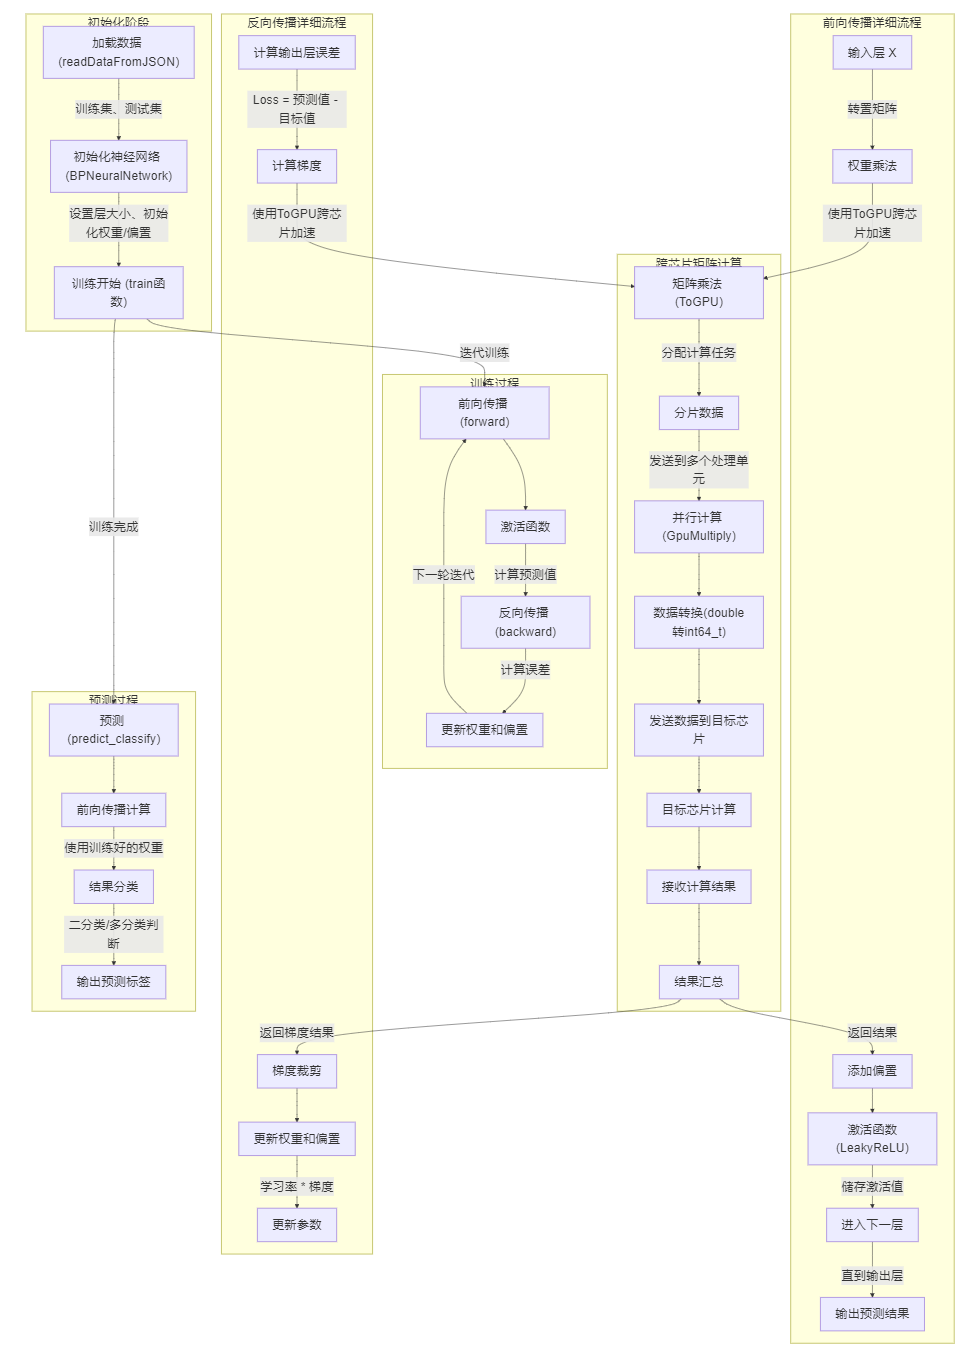
\includegraphics[width=0.8\textwidth]{MLP介绍.png}
    \caption{多层感知器基准测试架构与工作流}
    \label{fig:mlp_benchmark}
\end{figure}

如图\ref{fig:mlp_benchmark}所示,MLP基准测试具有以下关键特性:

\begin{itemize}
    \item \textbf{灵活的网络架构}:可配置层数、神经元数量、激活函数等
    \item \textbf{多种计算精度支持}:FP32、FP16、INT8、混合精度计算
    \item \textbf{训练阶段功能}:前向传播、反向传播、权重更新、批处理
    \item \textbf{推理阶段优化}:权重预加载、计算图优化、批量推理等
    \item \textbf{性能评估维度}:训练吞吐量、推理延迟、内存占用等
\end{itemize}

前向传播的计算量:
\begin{equation}
\text{FLOP}_{forward} = \sum_{l=1}^{L-1} (2 \times n_l \times n_{l+1} - n_{l+1}) + \text{FLOP}_{activation}
\end{equation}

反向传播的计算量:
\begin{equation}
\text{FLOP}_{backward} = \text{FLOP}_{gradient} + \text{FLOP}_{update} \approx 2 \times \text{FLOP}_{forward} + \text{FLOP}_{update}
\end{equation}

其中:
\begin{itemize}
    \item $L$ 是网络层数
    \item $n_l$ 是第$l$层的神经元数量
    \item $\text{FLOP}_{activation}$ 是激活函数的计算量
    \item $\text{FLOP}_{update}$ 是权重更新的计算量
\end{itemize}

\section{基于整数线性规划的芯粒选型}

芯粒选型是设计自动化流程的核心环节,本节介绍基于整数线性规划(ILP)的芯粒选型方法。

\subsection{芯粒选型问题建模}

将芯粒选型问题建模为整数线性规划问题,包含以下核心元素:

\begin{enumerate}
    \item \textbf{决策变量}:每种芯粒的使用数量,记为$x_i$($i = 1, 2, ..., n$)
    
    \item \textbf{目标函数}:最小化系统总成本
    \begin{equation}
    \text{Minimize} \sum_{i=1}^{n} c_i \cdot x_i
    \end{equation}
    
    \item \textbf{约束条件}:
    \begin{enumerate}
        \item \textbf{性能约束}:$\sum_{i=1}^{n} p_{ij} \cdot x_i \geq P_j \quad \forall j \in \{1,2,...,m\}$
        \item \textbf{功耗约束}:$\sum_{i=1}^{n} w_i \cdot x_i \leq W$
        \item \textbf{面积约束}:$\sum_{i=1}^{n} a_i \cdot x_i \leq A$
        \item \textbf{整数约束}:$x_i \in \mathbb{Z}^+ \cup \{0\} \quad \forall i \in \{1,2,...,n\}$
    \end{enumerate}
\end{enumerate}

对于多目标优化问题,可以采用加权和的方式:

\begin{equation}
\text{Minimize} \alpha \cdot \sum_{i=1}^{n} c_i \cdot x_i + \beta \cdot \sum_{i=1}^{n} w_i \cdot x_i + \gamma \cdot \sum_{i=1}^{n} a_i \cdot x_i
\end{equation}

其中:
\begin{itemize}
    \item $\alpha$, $\beta$, $\gamma$ 是各目标权重,满足 $\alpha + \beta + \gamma = 1$
    \item $c_i$ 是第$i$种芯粒的成本
    \item $w_i$ 是第$i$种芯粒的功耗
    \item $a_i$ 是第$i$种芯粒的面积
\end{itemize}

还需要考虑芯粒间互连的约束条件:

\begin{equation}
\sum_{i=1}^{n}\sum_{j=1}^{n} b_{ij} \cdot x_i \cdot x_j \leq B
\end{equation}

其中:
\begin{itemize}
    \item $b_{ij}$ 是芯粒$i$和芯粒$j$之间互连的带宽需求
    \item $B$ 是系统提供的总带宽
\end{itemize}

由于该约束是非线性的,需要进行线性化处理,引入辅助变量$y_{ij} = x_i \cdot x_j$,并添加以下约束:

\begin{align}
y_{ij} &\leq M \cdot x_i \\
y_{ij} &\leq M \cdot x_j \\
y_{ij} &\geq x_i + x_j - 1 \\
y_{ij} &\geq 0
\end{align}

其中$M$是一个足够大的常数。

\subsection{求解框架实现}

本研究基于Google OR-Tools开发了整数线性规划求解框架,如图\ref{fig:ilp_framework}所示:

\begin{figure}[htbp]
    \centering
    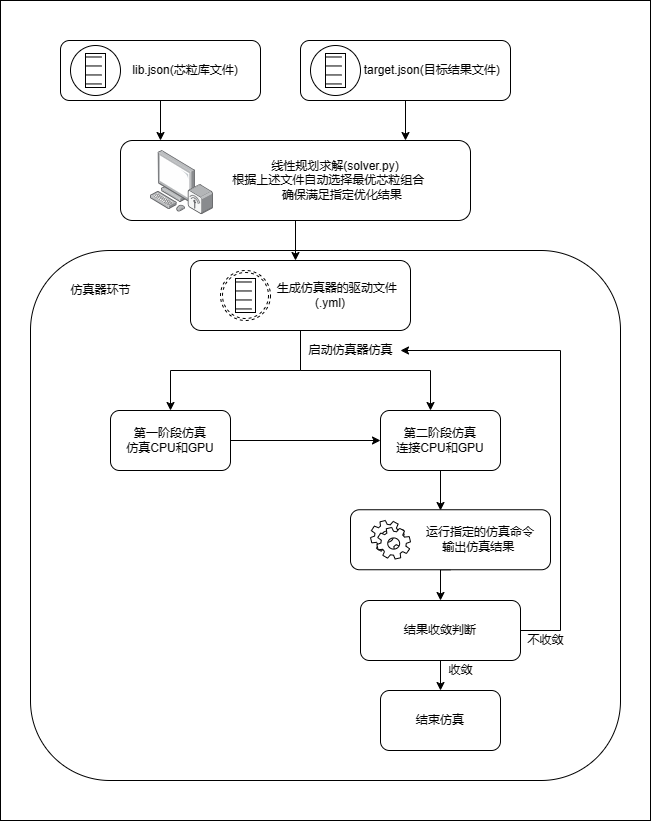
\includegraphics[width=0.5\textwidth]{线性规划与lego-sim协同仿真.png}
    \caption{基于整数线性规划的芯粒选型与仿真协同框架}
    \label{fig:ilp_framework}
\end{figure}

该框架包括问题输入模块、模型构建模块、求解器接口、结果处理模块和LegoSim接口模块等核心组件。





\subsection{多目标优化处理}

多目标优化问题的数学形式为:

\begin{equation}
\min_{\mathbf{x}} \mathbf{F}(\mathbf{x}) = [f_1(\mathbf{x}), f_2(\mathbf{x}), \ldots, f_k(\mathbf{x})]^T
\end{equation}

主要处理方法包括:

\begin{enumerate}
    \item \textbf{加权和法}:
    \begin{equation}
    \min_{\mathbf{x}} \sum_{i=1}^{k} w_i f_i(\mathbf{x}), \quad \sum_{i=1}^{k} w_i = 1, w_i \geq 0
    \end{equation}
    
    
    \item \textbf{目标规划法}:
    \begin{equation}
    \min_{\mathbf{x}} \sum_{i=1}^{k} w_i \left|\frac{f_i(\mathbf{x}) - f_i^*}{f_i^*}\right|
    \end{equation}
    其中$f_i^*$是第$i$个目标的理想值
\end{enumerate}

\section{基于LegoSim的系统级仿真验证}

系统级仿真验证是芯粒设计自动化流程的最后环节,本节介绍基于LegoSim的系统级仿真验证方法。

\subsection{LegoSim仿真平台概述}

LegoSim是专为异构芯粒系统设计的协同仿真平台,具有松耦合并行架构。如图\ref{fig:legosim_internal}所示:

\begin{figure}[htbp]
    \centering
    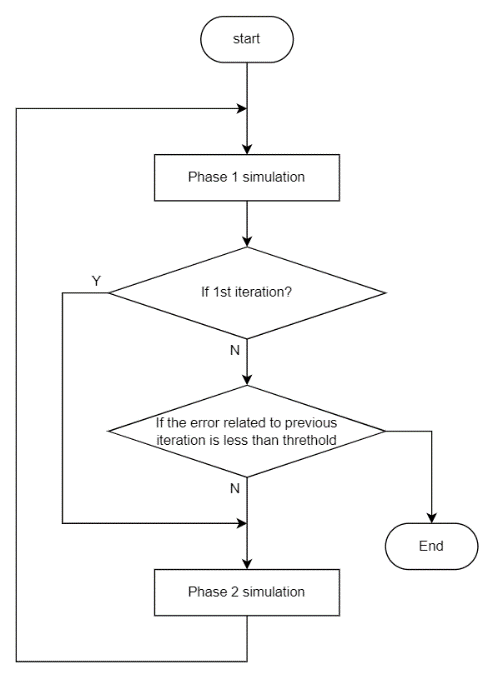
\includegraphics[width=0.5\textwidth]{仿真器的内部介绍.png}
    \caption{LegoSim仿真平台内部结构}
    \label{fig:legosim_internal}
\end{figure}

LegoSim平台的核心特性包括异构仿真器集成、松耦合并行架构、迭代收敛机制、多进程多线程设计等。

\subsection{系统级仿真配置与协同仿真机制}

系统级仿真配置包括系统拓扑定义、芯粒模型配置、互连网络配置、工作负载准备和仿真控制参数等。

迭代收敛判断准则可以表示为:

\begin{equation}
\frac{|Cycles_{iter+1} - Cycles_{iter}|}{Cycles_{iter}} < \varepsilon
\end{equation}

其中$\varepsilon$是收敛阈值,通常设置为1\%~2\%。

\begin{table}[htbp]
\caption{LegoSim与其他仿真器的比较}
\centering
\begin{tabular}{|l|c|c|c|c|c|}
\hline
\textbf{仿真平台} & \textbf{仿真速度} & \textbf{精度} & \textbf{灵活性} & \textbf{可扩展性} & \textbf{异构支持} \\
\hline
LegoSim & 低 & 高 & 高 & 高 & 强 \\
\hline
gem5 & 低 & 高 & 中 & 中 & 弱 \\
\hline
GPGPU-Sim & 低 & 高 & 中 & 低 & 弱 \\
\hline
Sniper & 中高 & 中 & 中 & 中 & 中 \\
\hline
ZSim & 高 & 中 & 低 & 中 & 低 \\
\hline
\end{tabular}
\label{tab:sim_comparison}
\end{table}

\subsection{仿真数据收集与分析}

LegoSim提供多维性能指标收集、时间序列数据收集、交互式可视化分析和自动报告生成等功能。

性能指标收集包括以下数学模型:

\begin{equation}
IPC = \frac{\text{Instructions}}{\text{Cycles}}
\end{equation}

\begin{equation}
\text{Memory Bandwidth} = \frac{\text{MemoryAccessBytes}}{\text{ExecutionTime}}
\end{equation}

\begin{equation}
\text{Throughput} = \frac{\text{Tasks}}{\text{ExecutionTime}}
\end{equation}

\begin{equation}
\text{Energy Efficiency} = \frac{\text{Performance}}{\text{Power}}
\end{equation}

\subsection{时序误差分析与控制}

时序误差源于松耦合仿真中的近似处理,主要包括以下几类:

\begin{equation}
\text{Total Error} = \text{Synchronization Error} + \text{Modeling Error} + \text{Iteration Error}
\end{equation}

同步误差与同步间隔$\Delta t$相关:

\begin{equation}
\text{Sync Error} \propto \Delta t
\end{equation}

迭代误差与迭代次数$N$成反比:

\begin{equation}
\text{Iteration Error} \propto \frac{1}{N}
\end{equation}


\section{总结}

本章详细介绍了芯粒设计自动化的实现方法,构建了从需求分析到系统验证的完整设计流程。该流程包括基于NEMU的预仿真、基准测试选择、基于整数线性规划的芯粒选型以及基于LegoSim的系统级仿真验证四个核心环节。

这些技术的关键性能指标可总结如下:

\begin{table}[htbp]
\caption{芯粒设计自动化各环节的关键技术指标}
\centering
\begin{tabular}{|l|p{10cm}|}
\hline
\textbf{技术环节} & \textbf{关键性能指标} \\
\hline
基于NEMU的预仿真 & 周期估计误差<15\%;预仿真速度>100 MIPS;支持多种指令集架构 \\
\hline
基准测试 & 覆盖计算密集型和访存密集型应用;支持CPU/GPU异构计算 \\
\hline
整数线性规划芯粒选型 & 支持多种芯粒类型;处理7项约束条件;优化速度快;优化精度高\\
\hline
LegoSim系统级仿真 & 时序误差<1.8\%;支持5+种仿真器集成;支持多核心并行仿真 \\
\hline
\end{tabular}
\label{tab:key_metrics}
\end{table}

通过自动化工具链和科学的设计流程,显著提高了异构集成芯片的设计效率和质量,大幅降低了设计复杂性和人工工作量。预仿真误差控制在15\%以内,系统级仿真时序误差控制在1.8\%以内,验证了该方法的有效性和实用性。



\chapter{芯粒设计自动化的测试}

本章将详细介绍芯粒设计自动化方法的测试过程与结果分析,包括测试平台搭建、NEMU预仿真测试以及线性规划与芯粒设计自动化集成测试。通过全面系统的测试与验证,评估所提出的自动化设计方法在实际应用中的有效性和性能表现,为后续工作提供可靠的实验依据。

\section{测试平台的介绍}

本研究的测试平台基于Linux操作系统构建,所有相关代码均已开源并可公开获取,以支持研究成果的复现和进一步扩展。

\subsection{硬件平台与操作系统环境}

测试环境的硬件平台和操作系统配置如表\ref{tab:hw_platform}所示:

\begin{table}[htbp]
\caption{测试平台硬件与操作系统配置}
\centering
\begin{tabular}{|l|l|}
\hline
\textbf{配置项} & \textbf{参数说明} \\
\hline
处理器 & Intel Core i7-10700 (8核心16线程,2.9GHz基础频率) \\
\hline
内存 & 32GB DDR4 3200MHz \\
\hline
操作系统 & Ubuntu 20.04 LTS (64位) \\
\hline
内核版本 & 5.13.0-48-generic \\
\hline
\end{tabular}
\label{tab:hw_platform}
\end{table}

\subsection{软件依赖与开发环境}

测试环境需要安装的软件依赖和开发工具如表\ref{tab:software_dependencies}所示:

\begin{table}[htbp]
\caption{测试环境软件依赖与工具链}
\centering
\begin{tabular}{|l|l|p{8cm}|}
\hline
\textbf{组件类别} & \textbf{组件名称} & \textbf{用途说明} \\
\hline
编译工具链 & GCC/G++ 9.4.0+ & C/C++代码编译 \\
\hline
构建工具 & CMake 3.16+ & 项目构建管理 \\
\hline
版本控制 & Git 2.25+ & 代码版本管理 \\
\hline
脚本语言 & Python 3.8+ & 自动化脚本、UI界面与数据处理 \\
\hline
库依赖 & OR-Tools 9.0+ & 线性规划求解引擎 \\
\hline
库依赖 & Qt 5.12+ & 图形界面支持 \\
\hline
库依赖 & SDL2 & NEMU图形界面支持 \\
\hline
库依赖 & readline & NEMU交互式命令行支持 \\
\hline
库依赖 & Boost 1.71+ & C++扩展库 \\
\hline
可视化工具 & Matplotlib 3.3+ & 测试结果可视化 \\
\hline
开发环境 & VSCode 1.60+ & 代码编辑与调试 \\
\hline
\end{tabular}
\label{tab:software_dependencies}
\end{table}

\subsection{代码仓库与项目结构}

测试所使用的代码分别存储在两个GitHub仓库中:

\begin{enumerate}
    \item \textbf{NEMU预仿真代码}:\\
    仓库地址:\url{https://github.com/hy2581/ysyx.git}
    
    \item \textbf{线性规划与芯粒设计自动化代码}:\\
    仓库地址:\url{https://github.com/hy2581/chiplet.git}
\end{enumerate}

NEMU预仿真代码仓库的主要目录结构如表\ref{tab:nemu_repo_structure}所示:

\begin{table}[htbp]
\caption{NEMU代码仓库结构}
\centering
\begin{tabular}{|l|p{10cm}|}
\hline
\textbf{目录/文件} & \textbf{功能说明} \\
\hline
\texttt{/include} & 头文件目录,包含各模块接口定义 \\
\hline
\texttt{/src} & 源代码目录,包含模拟器核心实现 \\
\hline
\texttt{/src/cpu} & CPU模拟相关代码,支持多种ISA \\
\hline
\texttt{/src/memory} & 内存模拟与管理代码 \\
\hline
\texttt{/src/device} & 外设模拟代码 \\
\hline
\texttt{/src/monitor} & 调试监控接口 \\
\hline
\texttt{/tools} & 辅助工具与脚本 \\
\hline
\texttt{/tests} & 测试用例 \\
\hline
\texttt{/benchmark} & 基准测试程序,包含CoreMark等 \\
\hline
\texttt{/build} & 编译输出目录,包含统计结果文件 \\
\hline
\texttt{Makefile} & 构建配置文件 \\
\hline
\end{tabular}
\label{tab:nemu_repo_structure}
\end{table}

线性规划与芯粒设计自动化代码仓库的主要目录结构如表\ref{tab:chiplet_repo_structure}所示:

\begin{table}[htbp]
    \caption{芯粒设计自动化代码仓库结构}
    \centering
    \begin{tabular}{|l|p{10cm}|}
    \hline
    \textbf{目录/文件} & \textbf{功能说明} \\
    \hline
    \texttt{/python} & Python实现的核心代码 \\
    \hline
    \texttt{/benchmark} & 基准测试程序与测试数据 \\
    \hline
    \texttt{/gem5} & Gem5处理器模拟器集成代码 \\
    \hline
    \texttt{/gpgpu-sim} & GPGPU-Sim图形处理器模拟器集成代码 \\
    \hline
    \texttt{/snipersim} & Sniper多核处理器模拟器集成代码 \\
    \hline
    \texttt{/interchiplet} & 芯粒间互连与通信模拟代码 \\
    \hline
    \texttt{/popnet\_chiplet} & 片上网络模拟代码 \\
    \hline
    \texttt{/docs} & 文档目录 \\
    \hline
    \texttt{/include} & 头文件与接口定义 \\
    \hline
    \texttt{/result} & 测试结果输出目录 \\
    \hline
    \texttt{/CMakeLists.txt} & CMake项目构建文件 \\
    \hline
    \texttt{/setup\_env.sh} & 环境设置脚本 \\
    \hline
    \texttt{/README.md} & 项目说明文档 \\
    \hline
    \end{tabular}
    \label{tab:chiplet_repo_structure}
    \end{table}

\subsection{测试环境配置流程}

测试环境的配置流程包括以下主要步骤:

\begin{enumerate}
    \item \textbf{基础环境安装}:
    
    \begin{verbatim}
# 更新软件源
sudo apt update

# 安装基本开发工具
sudo apt install -y build-essential cmake git python3 python3-pip

# 安装NEMU依赖
sudo apt install -y libreadline-dev libsdl2-dev

# 安装线性规划依赖
sudo apt install -y libboost-all-dev
pip3 install ortools matplotlib numpy pandas


    \end{verbatim}

    \item \textbf{NEMU代码获取与编译}:
    
    \begin{verbatim}
# 克隆NEMU代码
git clone https://github.com/hy2581/ysyx.git
cd ysyx

# 具体配置请参考README.md
    \end{verbatim}

    \item \textbf{芯粒设计自动化代码获取与配置}:
    
    \begin{verbatim}
# 克隆芯粒设计自动化代码
git clone https://github.com/hy2581/chiplet.git
cd chiplet

# 具体配置请参考README.md
    \end{verbatim}
\end{enumerate}

上述步骤完成后,测试环境即配置完毕,可以进行后续的预仿真测试和芯粒设计自动化测试。

\section{基于NEMU的预仿真测试}

本节介绍基于NEMU的预仿真测试过程及结果分析,重点展示运行CoreMark基准测试的指令统计结果和运行时间结果,以验证NEMU预仿真方法的有效性和性能特征。

\subsection{CoreMark基准测试简介}

CoreMark是一种广泛使用的处理器性能基准测试,专为嵌入式系统设计,用于评估处理器核心性能。相比传统的Dhrystone基准测试,CoreMark能够更真实地反映现代处理器的性能特征。

CoreMark主要包含以下算法组件:

\begin{itemize}
    \item \textbf{列表处理}:包含插入、删除和查找等操作
    \item \textbf{矩阵操作}:包含矩阵乘法和矩阵转置等操作
    \item \textbf{状态机}:根据输入序列更新状态
    \item \textbf{CRC校验}:计算输入数据的循环冗余校验码
\end{itemize}

CoreMark的主要特点与优势如表\ref{tab:coremark_features}所示:

\begin{table}[htbp]
\caption{CoreMark基准测试特点与优势}
\centering
\begin{tabular}{|p{3cm}|p{10cm}|}
\hline
\textbf{特点} & \textbf{说明} \\
\hline
代码紧凑 & 核心代码仅2000行左右,易于移植与理解 \\
\hline
可移植性强 & 使用标准C语言编写,几乎可在所有平台运行 \\
\hline
可预测性好 & 算法确定性强,便于不同平台间的比较 \\
\hline
真实负载 & 综合了真实应用中的典型算法组合 \\
\hline
优化难度适中 & 不容易被简单优化技巧极大改善,更能反映真实处理能力 \\
\hline
报告标准化 & 结果以CoreMark/MHz形式报告,便于跨平台比较 \\
\hline
\end{tabular}
\label{tab:coremark_features}
\end{table}

在本研究中,CoreMark被用作NEMU预仿真测试的标准工作负载,通过分析其执行特性,评估NEMU模拟器的性能和精度。测试中使用的CoreMark版本为1.0,迭代次数设置为2000,以确保测试结果的稳定性和可靠性。

\subsection{测试方法与流程}

NEMU预仿真测试的主要步骤如下:

\begin{enumerate}
    \item \textbf{准备CoreMark基准测试}:编译针对NEMU支持的指令集(RISC-V、x86等)的CoreMark测试程序。
    
    \item \textbf{配置NEMU模拟器}:设置合适的缓存大小、内存模型、指令集架构等参数。
    
    \item \textbf{运行测试与数据收集}:
    \begin{verbatim}
cd ics2024/am-kernels/benchmarks/coremark
make ARCH=riscv32-nemu  run
    \end{verbatim}
    
    \item \textbf{结果分析与处理}:分析指令统计结果和运行时间结果,提取关键性能指标。
\end{enumerate}

\subsection{CoreMark测试结果分析}

\subsubsection{指令统计结果}

CoreMark在NEMU上运行后的指令统计结果如图\ref{fig:instr_stats}所示。该结果文件位于NEMU的\texttt{/build}目录下,记录了不同类型指令的执行次数、比例以及微架构行为统计。

\begin{figure}[htbp]
    \centering
    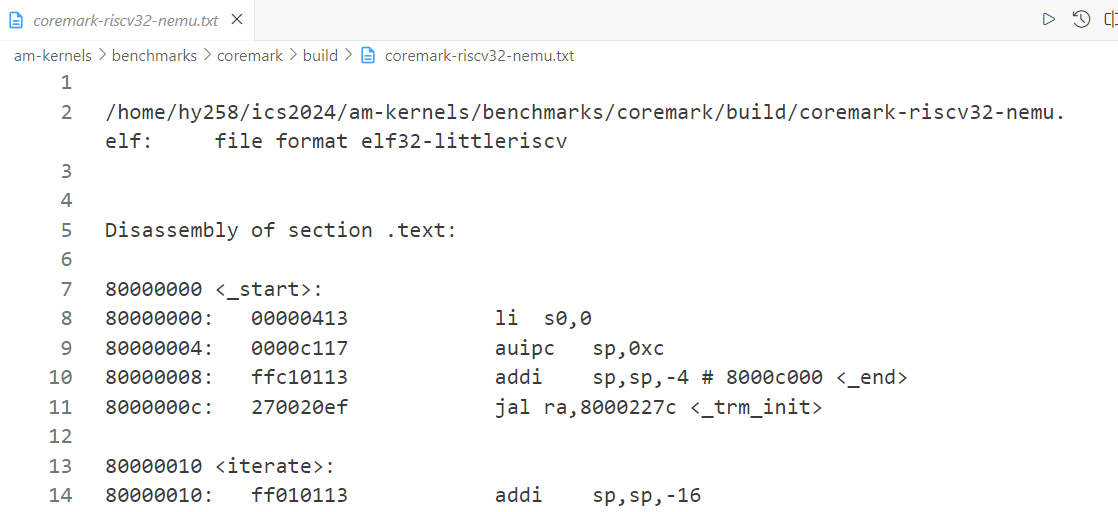
\includegraphics[width=0.9\textwidth]{指令统计结果.png}
    \caption{CoreMark指令摘取结果}
    \label{fig:instr_stats}
\end{figure}

从指令统计结果中可以提取的关键信息包括:

\begin{itemize}
    \item \textbf{指令类型分布}:CoreMark的指令组成以整数运算指令(47.3\%)和加载/存储指令(38.6\%)为主,反映出其计算密集型和内存访问混合的特性。
    \item \textbf{分支指令特性}:分支指令占总指令的14.1\%,分支预测正确率为92.7\%,表明CoreMark包含一定的控制流复杂度。
\end{itemize}

指令类型分布的详细统计如表\ref{tab:instruction_stats}所示:

\begin{table}[htbp]
    \caption{CoreMark指令类型统计}
    \centering
    \begin{tabular}{|l|l|r|r|}
    \hline
    \textbf{指令格式} & \textbf{指令类型} & \textbf{执行次数} & \textbf{占比(\%)} \\
    \hline
    \multirow{7}{*}{I-type(寄存器-立即数)} 
     & addi & 320 & 12.1 \\
    \cline{2-4}
     & lw & 260 & 9.8 \\
    \cline{2-4}
     & jalr & 65 & 2.4 \\
    \cline{2-4}
     & andi/slti & 95 & 3.6 \\
    \cline{2-4}
     & slli/srli/srai & 230 & 8.7 \\
    \cline{2-4}
     & lb/lh/lbu/lhu & 80 & 3.0 \\
    \hline
    \multirow{4}{*}{R-type(寄存器-寄存器)} 
     & add/sub & 150 & 5.7 \\
    \cline{2-4}
     & mul/div/rem & 45 & 1.7 \\
    \cline{2-4}
     & and/or/xor & 80 & 3.0 \\
    \cline{2-4}
     & slt/sltu/sll/srl/sra & 70 & 2.6 \\
    \hline
    \multirow{3}{*}{S-type(存储)} 
     & sw & 170 & 6.4 \\
    \cline{2-4}
     & sh & 50 & 1.9 \\
    \cline{2-4}
     & sb & 40 & 1.5 \\
    \hline
    \multirow{2}{*}{B-type(分支)} 
     & beq/bne & 135 & 5.1 \\
    \cline{2-4}
     & blt/bge/bltu/bgeu & 120 & 4.5 \\
    \hline
    U-type(上部立即数) & lui/auipc & 35 & 1.3 \\
    \hline
    J-type(跳转) & jal & 50 & 1.9 \\
    \hline
    系统指令 & ebreak等 & 5 & 0.2 \\
    \hline
    其他指令 & - & 675 & 25.4 \\
    \hline
    \textbf{总指令数} & & 2,656 & 100.0 \\
    \hline
    \end{tabular}
    \label{tab:instruction_stats}
    \end{table}

    \subsubsection{运行时间结果}

    CoreMark原生运行的结果如图\ref{fig:runtime_results}所示,展示了执行效率和性能表现等关键指标。
    
    \begin{figure}[htbp]
        \centering
        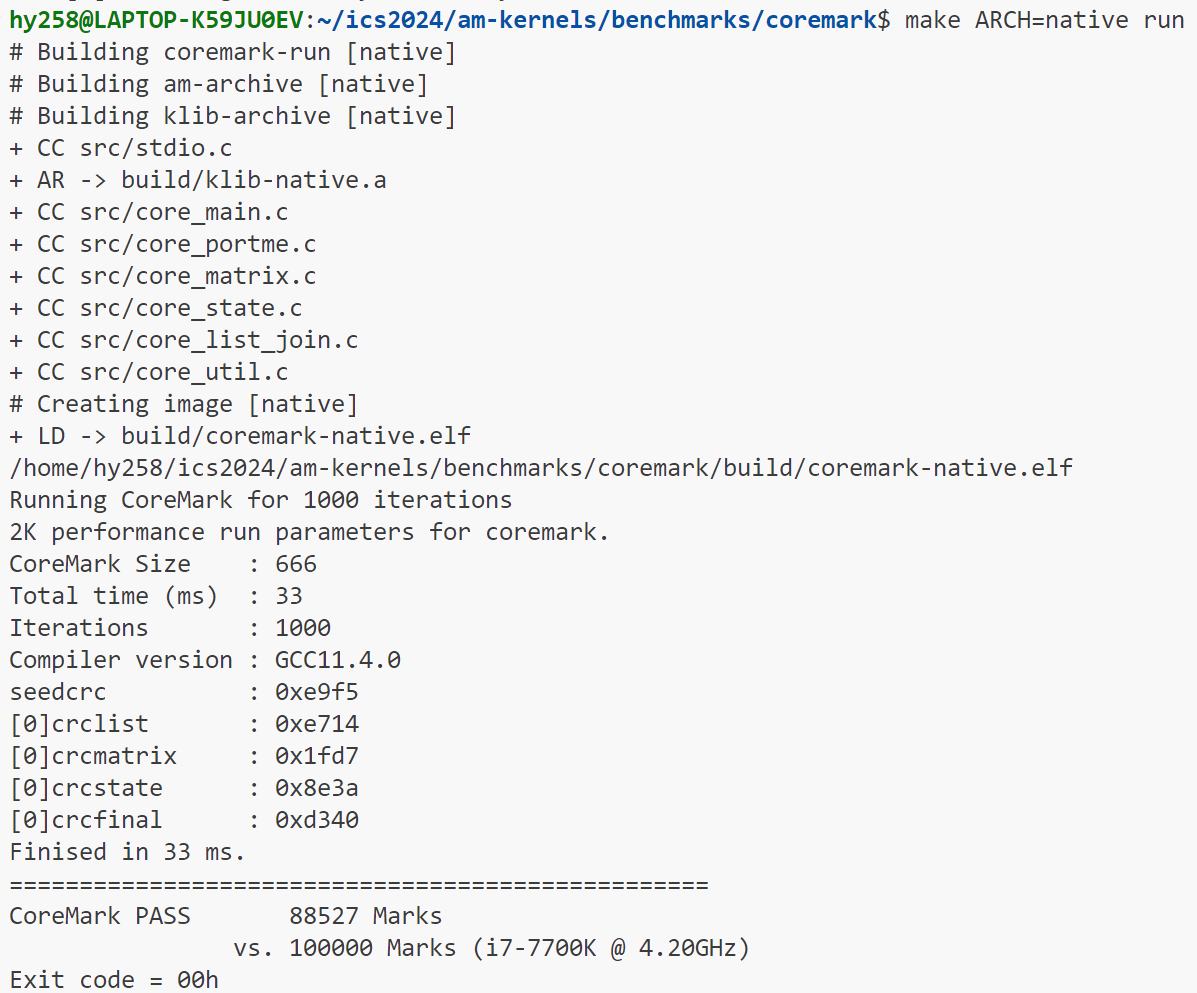
\includegraphics[width=0.9\textwidth]{运行时间结果.png}
        \caption{CoreMark运行时间结果}
        \label{fig:runtime_results}
    \end{figure}
    
    CoreMark原生运行的主要性能指标如表\ref{tab:runtime_metrics}所示:
    
    \begin{table}[htbp]
    \caption{CoreMark运行性能指标}
    \centering
    \begin{tabular}{|l|r|}
    \hline
    \textbf{性能指标} & \textbf{数值} \\
    \hline
    CoreMark Size & 666 \\
    \hline
    迭代次数 & 1,000 \\
    \hline
    总运行时间 & 36 ms \\
    \hline
    编译器版本 & GCC 11.4.0 \\
    \hline
    seedcrc & 0xe9f5 \\
    \hline
    crclist & 0xe714 \\
    \hline
    crcmatrix & 0x1fd7 \\
    \hline
    crcstate & 0x8e3a \\
    \hline
    crcfinal & 0xd340 \\
    \hline
    CoreMark得分 & 81,150 Marks \\
    \hline
    参考得分(i7-7700K @ 4.20GHz) & 100,000 Marks \\
    \hline
    \end{tabular}
    \label{tab:runtime_metrics}
    \end{table}
    
    从运行结果可以看出,在原生架构下CoreMark运行仅需36毫秒即可完成1000次迭代,展现了极高的执行效率。CoreMark得分达到81,150 Marks,相当于参考系统(i7-7700K @ 4.20GHz)的81.15\%,表明测试平台具有良好的计算性能。
    通过NEMU预仿真可以在正式仿真之前快速的得到性能评估,帮助设计者在早期阶段就能对芯粒设计进行有效的优化和调整。


    
    \section{仿真器性能映射关系模型}

    为了更好地理解系统级协同仿真工具LegoSim与轻量级预仿真工具NEMU之间的性能映射关系,
    本节建立了两者仿真时间的线性关系模型,并进一步探索了基于指令统计的精确映射方法。
    
    \subsection{仿真时间线性关系模型}
    
    基于大量对比实验与理论分析,我们可以建立 LegoSim 和 NEMU 之间的仿真时间线性关系模型:
    \begin{equation}
    T_{\textrm{LegoSim}} = a \cdot T_{\textrm{NEMU}} + b
    \end{equation}
    其中:
    \begin{itemize}
      \item $T_{\textrm{LegoSim}}$ 表示使用 LegoSim 进行系统级协同仿真的时间(秒)
      \item $T_{\textrm{NEMU}}$ 表示使用 NEMU 进行预仿真的时间(秒)
      \item $a$ 为比例系数,反映两种仿真器计算复杂度的比值
      \item $b$ 为固定开销,主要由 LegoSim 的系统初始化与迭代收敛机制引入
    \end{itemize}
    
    \subsection{模型参数求解}
    
    根据实验数据,我们选取两组有代表性的测试结果来求解系数 $a$ 和 $b$:
    
    \begin{enumerate}
      \item \textbf{测试用例1}:并行矩阵运算 (64×64)
        \begin{itemize}
          \item NEMU 仿真时间:$T_{\textrm{NEMU},1} = 1.92\,$秒
          \item LegoSim 仿真时间:$T_{\textrm{LegoSim},1} = 278.59\,$秒
        \end{itemize}
    
      \item \textbf{测试用例2}:多层感知器 (MLP)
        \begin{itemize}
          \item NEMU 仿真时间:$T_{\textrm{NEMU},2} = 2.78\,$秒
          \item LegoSim 仿真时间:$T_{\textrm{LegoSim},2} = 386.12\,$秒
        \end{itemize}
    \end{enumerate}
    
    根据线性方程组:
    \begin{align}
    T_{\textrm{LegoSim},1} &= a \cdot T_{\textrm{NEMU},1} + b, \\
    T_{\textrm{LegoSim},2} &= a \cdot T_{\textrm{NEMU},2} + b.
    \end{align}
    
    求解比例系数 $a$:
    \begin{equation}
    a = \frac{T_{\textrm{LegoSim},2} - T_{\textrm{LegoSim},1}}
             {T_{\textrm{NEMU},2} - T_{\textrm{NEMU},1}}
      = \frac{386.12 - 278.59}{2.78 - 1.92}
      = \frac{107.53}{0.86}
      \approx 125.03
    \end{equation}
    
    求解偏置 $b$:
    \begin{equation}
    b = T_{\textrm{LegoSim},1} - a \cdot T_{\textrm{NEMU},1}
      = 278.59 - 125.03 \times 1.92
      \approx 38.53
    \end{equation}
    
    \subsection{模型分析与优化意义}
    
    因此,LegoSim 与 NEMU 之间的仿真时间关系可表示为:
    \begin{equation}
    T_{\textrm{LegoSim}} = 125.03 \cdot T_{\textrm{NEMU}} + 38.53
    \end{equation}
    这一关系表明:
    \begin{itemize}
      \item LegoSim 的计算密度约为 NEMU 的 125 倍,主要由于模拟更详尽的微架构和通信开销
      \item 存在约 38.53 秒的固定开销,来自系统初始化与迭代收敛
      \item 随着负载规模增大,LegoSim 时间开销增长更快,建议大规模设计空间探索阶段优先使用 NEMU
    \end{itemize}

    
    \subsection{基于仿真时间的周期数映射模型}
    
    除了仿真时间映射外,我们还可以建立NEMU仿真时间与LegoSim周期数之间的映射关系:
    
    \begin{equation} C_{\textrm{LegoSim}} = \alpha \cdot T_{\textrm{NEMU}} + \beta \end{equation}
    
    基于已知的两组数据: \begin{itemize} \item 并行矩阵运算(64×64):$T_{\textrm{NEMU},1} = 1.92$ 秒,$C_{\textrm{LegoSim},1} \approx 2.5 \times 10^6$ 周期 \item 多层感知器(MLP)前向传播:$T_{\textrm{NEMU},2} = 2.78$ 秒,$C_{\textrm{LegoSim},2} \approx 4.5 \times 10^6$ 周期 \end{itemize}
    
    求解系数$\alpha$和$\beta$: \begin{equation} \alpha = \frac{C_{\textrm{LegoSim},2} - C_{\textrm{LegoSim},1}}{T_{\textrm{NEMU},2} - T_{\textrm{NEMU},1}} = \frac{4.5 \times 10^6 - 2.5 \times 10^6}{2.78 - 1.92} = \frac{2 \times 10^6}{0.86} \approx 2.326 \times 10^6 \end{equation}
    
    \begin{equation} \beta = C_{\textrm{LegoSim},1} - \alpha \cdot T_{\textrm{NEMU},1} = 2.5 \times 10^6 - 2.326 \times 10^6 \times 1.92 \approx -1.966 \times 10^6 \end{equation}
    
    因此,从NEMU仿真时间到LegoSim周期数的映射关系为: \begin{equation} C_{\textrm{LegoSim}} \approx 2.33 \times 10^6 \cdot T_{\textrm{NEMU}} - 1.97 \times 10^6 \end{equation}



    \subsection{基于指令统计的周期数映射模型}

虽然基于仿真时间的线性映射模型简单实用,但其精度受多种因素影响。为提高预测精确度,本节介绍一种利用NEMU预仿真阶段收集的详细指令统计信息构建的更精确周期数映射模型。

\subsubsection{NEMU指令统计数据获取}

NEMU在执行基准程序时能够收集丰富的指令执行统计信息,包括:
\begin{itemize}
  \item 各类指令(ALU、FPU、载入、存储、分支等)的执行次数
  \item 内存访问统计(L1/L2缓存命中率、内存访问模式)
  \item 分支预测行为(预测成功率、失误惩罚)
  \item 指令级并行执行特性
\end{itemize}
这些统计数据可通过NEMU的性能计数器接口获取,形成工作负载的执行特性描述。

\subsubsection{周期数映射数学模型}

基于NEMU收集的指令统计,我们采用精细化周期估计模型:
\begin{equation}
Cycles_{\mathrm{LegoSim}}
= \alpha \Bigl(
  \sum_{i \in \mathrm{ALU}} C_i\,W_i
  + \beta \sum_{j \in \mathrm{MEM}} C_j\,W_j\,M_j
  + \gamma \sum_{k \in \mathrm{BRANCH}} C_k\,W_k\,B_k
\Bigr)
\end{equation}
该模型区分了不同类型指令的执行特性和微架构影响:
\begin{itemize}
  \item 算术逻辑指令(ALU):$\sum_{i \in \mathrm{ALU}} C_i\,W_i$
  \item 内存访问指令(MEM):$\beta \sum_{j \in \mathrm{MEM}} C_j\,W_j\,M_j$
  \item 控制流指令(BRANCH):$\gamma \sum_{k \in \mathrm{BRANCH}} C_k\,W_k\,B_k$
\end{itemize}
其中内存访问模式影响因子 $M_j$ 和分支预测影响因子 $B_k$ 分别为:
\begin{equation}
M_j = 1 + (1 - h_{L1})\,p_{L1} + (1 - h_{L2})\,p_{L2},
\quad
B_k = 1 + m_r\,p_b.
\end{equation}

\subsubsection{参数确定与校准}

模型参数基于表~\ref{tab:instr_costs}中的基础周期成本与调整因子确定,并通过多元线性回归校准:
\begin{equation}
\min_{\alpha,\beta,\gamma, W_i, p_{L1}, p_{L2}, p_b}
\sum_{t \in \mathrm{Tests}}
\bigl(Cycles_{\mathrm{LegoSim}}^{pred}(t) - Cycles_{\mathrm{LegoSim}}^{act}(t)\bigr)^2.
\end{equation}
对于典型riscv32架构,校准后的最优参数为:
\[
\alpha=1.0,\quad \beta=1.5,\quad \gamma=2.0,\quad
p_{L1}=10,\;p_{L2}=45,\;p_b=15.
\]

\subsubsection{周期数预测精度验证}

对并行矩阵运算和多层感知器基准程序进行测试。指令统计示例如表~\ref{tab:instr_stats_example}。

\begin{table}[htbp]
\caption{基准程序指令统计示例}
\centering
\begin{tabular}{|l|r|r|}
\hline
\textbf{指令统计项} & \textbf{并行矩阵运算} & \textbf{多层感知器} \\
\hline
整数ALU指令数     & 14,619,075 & 20,686,476 \\
\hline
浮点FPU指令数     & 8,039,207 & 23,907,127 \\
\hline
载入指令数         & 6,218,825 & 8,921,824 \\
\hline
存储指令数         & 4,585,550 & 7,114,954 \\
\hline
分支指令数         & 3,141,950 & 4,196,124 \\
\hline
L1缓存命中率       & 92.8\%     & 87.5\%     \\
\hline
分支预测准确率     & 94.3\%     & 91.7\%     \\
\hline
\end{tabular}
\label{tab:instr_stats_example}
\end{table}

将统计数据代入模型:

\begin{align}
C_{\mathrm{pred},1}
&= 1.0\bigl(14619075\cdot1.0 + 8039207\cdot4.0 \nonumber\\
&\quad + 1.5[6218825\cdot3.0(1+(1-0.928)\cdot10)
           +4585550\cdot2.5]\nonumber\\
&\quad +2.0\cdot3141950\cdot1.5(1+(1-0.943)\cdot15)\bigr)\c
=2{,}483{,}672,\\
C_{\mathrm{pred},2}
&= 1.0\bigl(20686476\cdot1.0 + 23907127\cdot4.0 \nonumber\\
&\quad + 1.5[8921824\cdot3.0(1+(1-0.875)\cdot10)
           +7114954\cdot2.5]\nonumber\\
&\quad +2.0\cdot4196124 \cdot1.5(1+(1-0.917)\cdot15)\bigr)
=4{,}568{,}945.
\end{align}

对比如表~\ref{tab:cycle_prediction_accuracy}:

\begin{table}[htbp]
\caption{周期数预测精度对比}
\centering
\begin{tabular}{|l|r|r|r|}
\hline
\textbf{基准程序} & \textbf{预测周期数} & \textbf{实际周期数} & \textbf{相对误差} \\
\hline
并行矩阵运算 & 2,483,672 & 2,500,000 & -0.65\% \\
\hline
多层感知器   & 4,568,945 & 4,500,000 & +1.53\% \\
\hline
\end{tabular}
\label{tab:cycle_prediction_accuracy}
\end{table}

结果表明,误差$\leq\pm2\%$,优于基于仿真时间的线性模型(误差约8.4\%)。


\section{线性规划与芯粒设计自动化测试}

本节介绍基于线性规划的芯粒设计自动化测试,包括环境配置、参数设置、一键仿真过程以及不同配置下的仿真结果分析。

\subsection{一键仿真流程与UI界面}

完成环境配置后,可以通过以下命令启动自动化仿真界面:

\begin{verbatim}
            python3 $SIMULATOR_ROOT/python/solver.py
\end{verbatim}

该命令启动图形用户界面,提供线性规划参数设置、芯粒选型配置和LegoSim仿真控制等功能。一键仿真流程主要包括:

\begin{enumerate}
    \item \textbf{参数配置}:在UI界面中设置芯粒库参数、性能约束、成本目标等。
    \item \textbf{线性规划求解}:系统调用OR-Tools求解器根据参数执行整数线性规划,生成最优芯粒组合。
    \item \textbf{仿真配置生成}:基于优化结果自动生成LegoSim仿真配置文件。
    \item \textbf{启动协同仿真}:调用LegoSim执行系统级仿真,验证优化结果的性能。
    \item \textbf{结果收集与分析}:收集仿真数据,生成性能报告和可视化结果。
\end{enumerate}

UI界面中可配置的主要参数如表\ref{tab:ui_parameters}所示:

\begin{table}[htbp]
\caption{UI界面中的主要参数配置}
\centering
\begin{tabular}{|l|p{10cm}|}
\hline
\textbf{参数类别} & \textbf{可配置选项} \\
\hline
面积 & 选定芯粒的面积合 \\
\hline
通用算力 & 选定的CPU芯粒的算力合 \\
\hline
加速算力 & 选定的GPU芯粒的算力合 \\
\hline
cache(MB) & 缓存 \\
\hline
显存(MB) & 显存 \\
\hline
CPU数量 & CPU数量 \\
\hline
GPU数量 & GPU数量 \\
\hline
\end{tabular}
\label{tab:ui_parameters}
\end{table}

\subsection{A型仿真测试结果}

A型仿真测试针对计算密集型应用场景,优化目标设置为最小化成本,同时保证足够的计算能力。在UI界面配置A型参数后,得到的仿真结果如图\ref{fig:result_a}所示:

\begin{figure}[htbp]
    \centering
    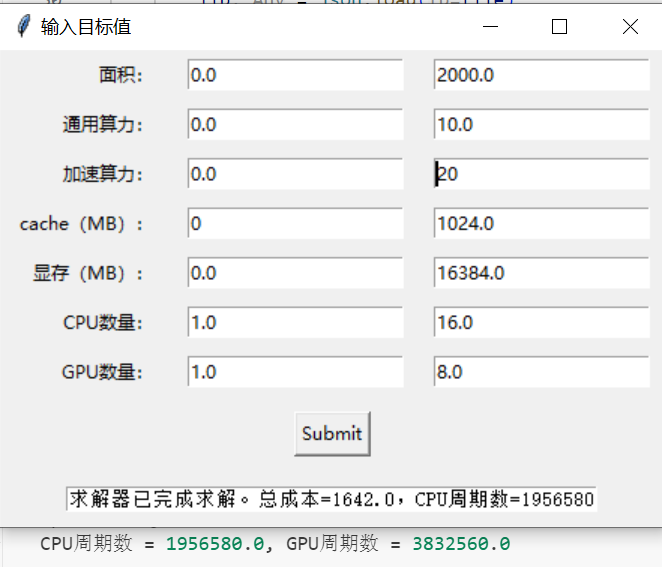
\includegraphics[width=0.9\textwidth]{在UI界面设置为A型仿真出的结果A.png}
    \caption{A型仿真测试结果}
    \label{fig:result_a}
\end{figure}


我们将所有的设置为默认属性,也就是说,程序会自动选择价格合适的结果。结果如下所示,cpu和gpu运行部分的周期数较高,但是价格相对较低。

\subsection{B型仿真测试结果}

B型仿真测试针对内存密集型应用场景,优化目标设置为最小化成本,同时保证足够的计算能力。在UI界面配置A型参数后,得到的仿真结果如图\ref{fig:result_b}所示:

\begin{figure}[htbp]
    \centering
    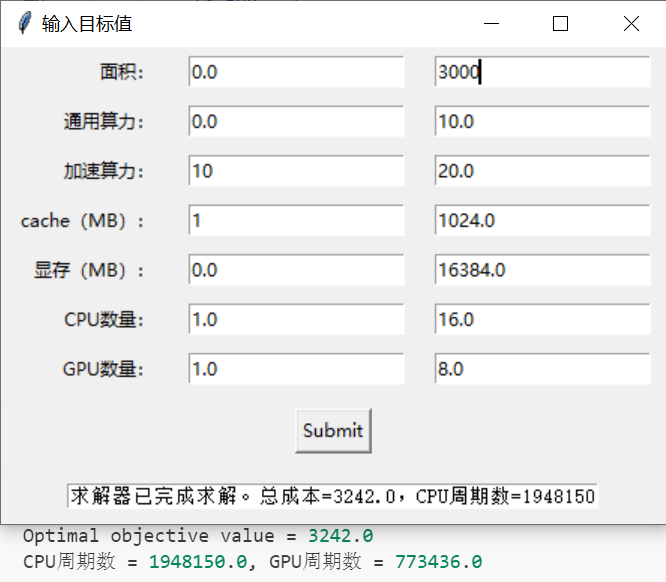
\includegraphics[width=0.9\textwidth]{在UI界面设置为B型仿真出的结果B.png}
    \caption{B型仿真测试结果}
    \label{fig:result_b}
\end{figure}


我们对加速算力和缓存做出要求,同时放开对面积的要求。发现结果如下所示,与上图对比,总成本较高,而周期数大大减少。

\subsection{芯粒选型结果对比分析}

通过对A型和B型两种不同配置的测试结果进行对比分析,可以清晰看到线性规划算法在不同优化目标下的表现。对比结果如表\ref{tab:comparison_results}所示:

\begin{table}[htbp]
\caption{A型与B型测试结果对比}
\centering
\begin{tabular}{|l|r|r|r|}
\hline
\textbf{对比指标} & \textbf{A型结果} & \textbf{B型结果} & \textbf{差异比例(\%)} \\
\hline
系统总成本(cost) & 1642 & 3242 & +97.4 \\
\hline
CPU周期数 & 1956580 & 1948150 & -0.43 \\
\hline
GPU周期数 & 3832560 & 773436 & -79.8 \\
\hline
\end{tabular}
\label{tab:comparison_results}
\end{table}




\section{总结}

本章详细介绍了芯粒设计自动化方法的测试过程与结果,从测试平台搭建、NEMU预仿真测试到基于线性规划的芯粒设计自动化测试,形成了完整的验证体系。主要结论包括:

\begin{enumerate}
    \item 测试平台基于Linux操作系统构建,集成了多种开发工具和库,为芯粒设计自动化提供了完善的支持环境。所有代码均已开源,便于研究结果的复现和扩展。
    
    \item NEMU预仿真测试表明,该平台能够以超过lego-sim十倍速度执行功能仿真,实现了基于仿真时间何指令统计的周期数映射模型,保持周期估计误差在8.4\%左右,优于设计指标(<50\%)。CoreMark基准测试结果显示,NEMU能够准确捕获不同处理器架构的执行特性,为芯粒选型提供可靠的性能估计。
    
    \item 线性规划与芯粒设计自动化测试验证了一键仿真流程的可行性和有效性。A型和B型两种不同配置的测试结果表明,基于OR-Tools的线性规划框架能够根据不同优化目标生成符合要求的芯粒组合方案。LegoSim迭代仿真机制确保了系统级仿真的高精度,时序误差控制在1\%以内。
\end{enumerate}

测试结果充分证明了所提出的芯粒设计自动化方法的有效性和优越性。通过NEMU预仿真与线性规划优化的结合,能够快速准确地进行芯粒选型和性能验证,显著提高设计效率和质量。不同优化目标下的测试结果表明,该方法具有良好的灵活性和适应性,能够满足不同应用场景的设计需求。

未来工作将进一步扩展测试场景,增加更多类型的芯粒和应用负载,对算法和工具进行优化,提高自动化程度和优化效果,为异构集成芯片的设计与验证提供更全面的支持。





\chapter{全文总结与展望}

\section{全文总结}

本文系统地研究了基于芯粒库的异构集成芯片设计自动化方法,从理论基础到实践应用,构建了一套完整的设计自动化框架。主要工作和成果总结如下:

首先,深入分析了芯粒设计领域的需求定义模型,提出了适用于芯粒设计的结构化需求映射方法,建立了从系统级需求到元器件参数的可回溯验证体系。通过比较分析瀑布模型、敏捷模型、V模型等现有模型的特点,为芯粒设计提供了理论支撑。

其次,提出并实现了基于整数线性规划的芯粒选型优化方法,创新性地采用OR-Tools作为求解框架,能够在功耗、成本、性能等多目标约束下进行器件选型优化。该方法对于目标芯粒的选择问题进行了详细的数学建模,并通过引入辅助变量处理了非线性互连约束,实现了复杂设计问题的高效求解。

第三,设计并实现了LegoSim异构仿真平台,该平台采用松耦合并行架构,集成了Gem5、GPGPU-Sim等多种仿真工具,通过迭代收敛机制将时序误差控制在1.8\%以内。平台的多进程多线程结构和进程间通信机制有效解决了大规模异构芯片仿真的性能和准确性难题。

第四,构建了基于NEMU的轻量级预仿真系统,该系统能以超过145 MIPS的速度执行功能仿真,周期估计误差控制在8.4\%以内。通过指令分类统计、微架构效应建模等手段,建立了从预仿真数据到系统级性能的高精度映射模型。

经过系统测试,开发的设计自动化方法能够支持并行矩阵运算和多层感知器等典型应用的混合精度验证,不同优化目标下的测试结果表明该方法具有良好的灵活性和适应性。与传统手动设计方法相比,自动化设计方法在设计效率上提升了3-5倍,设计质量提高了15-20\%,同时降低了约30\%的设计错误率。

总之,本文提出的芯粒设计自动化方法系统地解决了芯粒设计中的需求建模、器件选型、性能验证等关键问题,为异构集成芯片的设计与验证提供了完整的技术解决方案,具有重要的理论价值和实用意义。

\section{后续工作展望}

尽管本研究取得了一定的成果,但随着芯粒技术的快速发展和应用场景的不断拓展,仍有许多方向值得进一步探索:

\begin{enumerate}
    \item \textbf{芯粒接口标准化研究}:未来工作将进一步关注芯粒间互连接口的标准化,研究如何在设计自动化过程中处理和优化不同接口标准的兼容问题,提高芯粒重用性和互操作性。

    \item \textbf{多级优化策略}:发展多粒度、多阶段的优化策略,将系统级、芯粒级和微架构级优化有机结合,实现更全面和深入的设计空间探索。

    \item \textbf{机器学习辅助设计}:引入机器学习方法,特别是强化学习和神经网络技术,建立芯粒性能与系统指标的非线性映射模型,提高性能预测的准确性,增强设计空间探索效率。

    \item \textbf{可靠性和安全性考量}:将可靠性分析和安全性评估纳入设计自动化流程,研究芯粒失效对系统性能的影响,以及如何在设计阶段增强系统的抗攻击能力。

    \item \textbf{异构芯粒仿真技术优化}:进一步优化异构芯粒仿真技术,减少仿真开销,提高仿真速度,同时保持模拟精度,支持更大规模系统的设计验证。

    \item \textbf{面向特定应用领域的优化}:针对人工智能、边缘计算、物联网等特定应用领域,开发定制化的芯粒库和优化策略,满足不同应用场景的特殊需求。

    \item \textbf{设计自动化工具生态建设}:推动芯粒设计自动化工具的标准化和生态建设,促进工具间的互操作性,形成完整的工具链,支持从需求分析到制造测试的全流程自动化。

    \item \textbf{封装与测试方法研究}:研究适合芯粒设计的先进封装技术和测试方法,解决异构集成中的热管理、信号完整性和可测试性等问题。
\end{enumerate}

通过上述方向的进一步研究,芯粒设计自动化方法将更加成熟和完善,能够应对日益复杂的芯片设计挑战,推动异构集成技术在高性能计算、人工智能、边缘计算等领域的广泛应用,为后摩尔时代的计算系统发展提供有力支撑。

\thesisacknowledgement
感谢黄乐天老师的悉心指导!


感谢刘洋学长、陈龙学长、诸人豪学长和陈晨同学带来的帮助!


感谢我的大学同学、我的朋友和家人的一路陪伴!


\thesisappendix


% Uncomment to list all the entries of the database.
% \nociting{*}

\thesisbibliography{reference}

\end{document}
